\documentclass[a4paper,11pt,twoside]{ThesisStyle}

\include{formatAndDefs}

\begin{document}

\begin{titlepage}

% $\raise\baselineskip\hbox{
%    \vtop to0pt{%
%       \hbox{}\hbox to0pt{
\includegraphics[scale=0.14]{tlloria}\hss}\vss}%
% }$\hskip2.5cm%




\begin{center}

\noindent {\large \textbf{UNIVERSITY OF FRANCHE-COMTE}} \\
\vspace*{0.3cm}
\noindent {\LARGE \textbf{DOCTORAL SCHOOL SPIM}} \\
\noindent \textbf{LABORATOIRE D'INFORMATIQUE DE L'UNIVERSITE DE FRANCHE-COMTE\\ (LIFC) } \\
\vspace*{0.5cm}
\noindent \Huge \textbf{P H D\ \ T H E S I S} \\
\vspace*{0.3cm}
\noindent \large {to obtain the title of} \\
\vspace*{0.3cm}
\noindent \LARGE \textbf{PhD of Science} \\
\vspace*{0.3cm}
\noindent \Large of the University of Franche-Comte \\
\noindent \Large \textbf{Specialty : \textsc{Computer Science}}\\
\vspace*{0.4cm}
\noindent \large {Defended by\\}
\noindent \LARGE Qianxue \textsc{WANG} \\
\vspace*{0.8cm}
\noindent {\Huge \textbf{Generating pseudo-random numbers. Applications in cryptology}} \\
\vspace*{0.8cm}
\noindent \Large Thesis Advisor:  Jacques \textsc{Bahi} \\
\vspace*{0.2cm}
\noindent \Large prepared at Numerical and Distributed Algorithms: \textsc{AND} Team\\
\vspace*{0.2cm}
\noindent \large defended on February 28, 2011 \\
\vspace*{0.5cm}
\end{center}
\noindent \large \textbf{Jury :} \\
\begin{center}
\noindent \large 
\begin{tabular}{llcl}
      \textit{Reviewers :}	&   \textsc{ }		& - &   \\
				&   \textsc{ }		& - &  \\
      \textit{Advisor :}	&  \textsc{}		& - &  \\
      \textit{President :}	&  \textsc{}		& - & \\
      \textit{Examinators :}   &  \textsc{}          & - & \\
      				&  \textsc{}			& - & \\
      				& \textsc{}		& - & \\
      \textit{Invited :}		&  \textsc{}		& - & 
\end{tabular}
\end{center}

% \newcommand{\@NancyIhe@d}{{\UseEntryFont{ThesisFirstPageHead}\noindent
%     \centerline{\if@logo@uhp@
%                     {\setbox0=\hbox{$\raise2.5cm\hbox{\UHPLogo}$}%
%                      \ht0=\baselineskip\box0}\hfill
%                 \else
%                     Universit\'e Henri Poincar\'e -- Nancy 1%
%                 \fi}%
%     \@TL@cmn@head\\
%     UFR ST\par
%     }%
%     }
% \hbox{$\raise2.5cm\hbox{\vtop to0pt{\hbox{}\hbox to0pt{
\includegraphics[scale=0.2]{tluhp}\hss}\vss}$}

\end{titlepage}
\sloppy

\titlepage


\dominitoc

\pagenumbering{roman}

 \cleardoublepage

\section*{Acknowledgments}

Last thing to do :-)

% Technical support from Le m\'esocentre de calcul de Franche-Comt\'e is gratefully acknowledged. 
% We are also grateful to Xiaole Fang for the calculations of Comparative test parameters and Kamel Mazouzi for his helpful comments on cluster computing.

\tableofcontents

\mainmatter

\include{Introduction}

\include{ReviewofBasics}


\include{DesignofCIPRNG}


\include{StatisticalTestsforRandomness}


\chapter{Performance Evaluation}
\label{Performance Evaluation}
\minitoc

Although non-uniform distributed random numbers may be needed in some applications,
for example the user request generator with non-uniform distributed arrival rate in a queuing
system, it is still a majority to have a random sequence with uniform distribution over certain
domain S (this kind of random number generator is called uniform random number generator). 
In order to test the uniformity of a sequence, several methods can be applied.

\section{Balance of Probability}


If a bit sequence is concerned, the uniformity can be justified by comparing the
number of 0's and 1's appeared. That can be accounted with the balance of probability [19],
which defined as$\frac{p-q}{n}$, where $p$ and $q$ are the occurrence frequencies of ``1`` and ``0``,
respectively and $n$ is the number of bits. Figure~\ref{Balance of Probability for old CI} and Figure~\ref{Balance of Probability for new CI} show the balance of probability for a bit
sequence generated by chaotic iterations, showing that the chances to have ``0`` and ``1`` are more or less
the same.
\begin{figure}
\centering
\subfigure[Old CI(Logistic, Logistic)]{\includegraphics[scale=0.34]{images/balance_oldci_ll.eps}
} \hspace{0.5cm}
\subfigure[Old CI(XORshift, XORshift)]{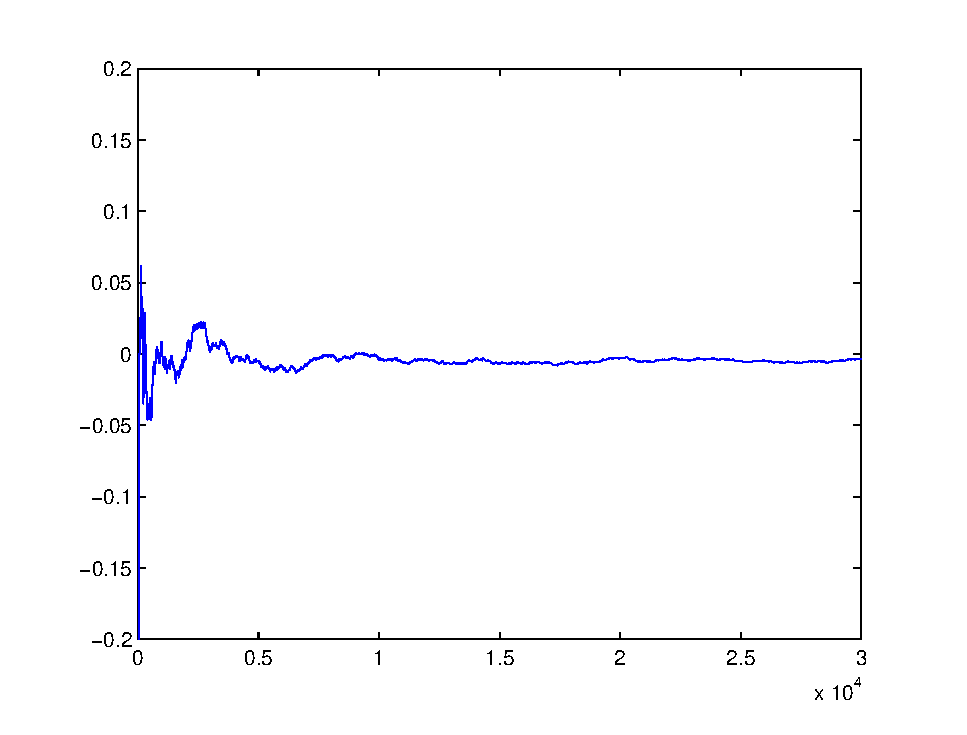
\includegraphics[scale=0.34]{images/balance_oldci_xx.eps}
} \hspace{0.5cm}
\subfigure[Old CI(ISAAC, XORshift)]{\includegraphics[scale=0.34]{images/balance_oldci_xi.eps}
} \hspace{0.5cm}
\subfigure[Old CI(ISAAC, ISAAC)]{\includegraphics[scale=0.34]{images/balance_oldci_ii.eps}
} \hspace{0.5cm}
\caption{Balance of Probability for old CI}
\label{Balance of Probability for old CI}
\end{figure}

\begin{figure}
\centering
\subfigure[New CI(XORshift, XORshift)]{\includegraphics[scale=0.34]{images/balance_newci_xx.eps}
} \hspace{0.5cm}
\subfigure[New CI(ISAAC, XORshift)]{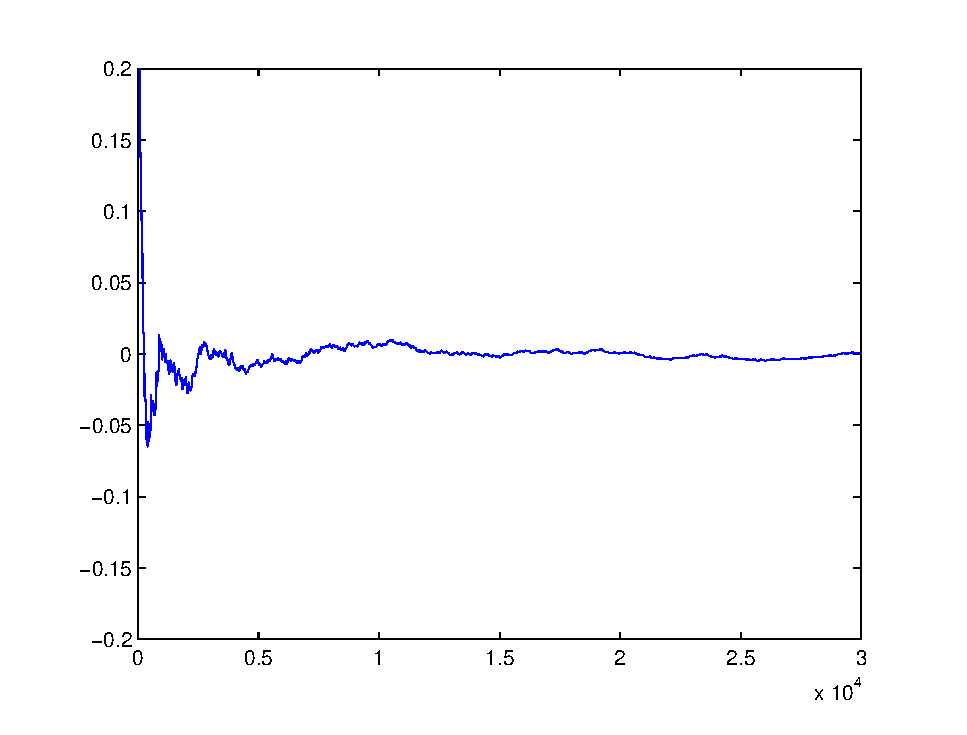
\includegraphics[scale=0.34]{images/balance_newci_xi.eps}
} \hspace{0.5cm}
\subfigure[New CI(ISAAC, ISAAC)]{\includegraphics[scale=0.34]{images/balance_newci_ii.eps}
} \hspace{0.5cm}
\caption{Balance of Probability for new CI}
\label{Balance of Probability for new CI}
\end{figure}

\section{Sensitivity}

As a consequence of its chaotic property, this PRNG is highly sensitive to the initial conditions. To illustrate this property, several initial values are put into the chaotic system. Let $H$ be the number 
of differences between the sequences obtained in this way. Suppose $n$ is the length of these 
sequences. Then the variance ratio $P$, defined by $P = H / n$, is computed. The results are 
shown in Figure~\ref{Sensitivity for old CI} and Figure~\ref{Sensitivity for new CI} ($x$ axis is sequence lengths, $y$ axis is variance ratio $P$). For the two PRNGs, variance 
ratios approach $0.50$, which indicate that the systems are extremely sensitive to the initial 
conditions.
\begin{figure}
\centering
\subfigure[Old CI(Logistic, Logistic)]{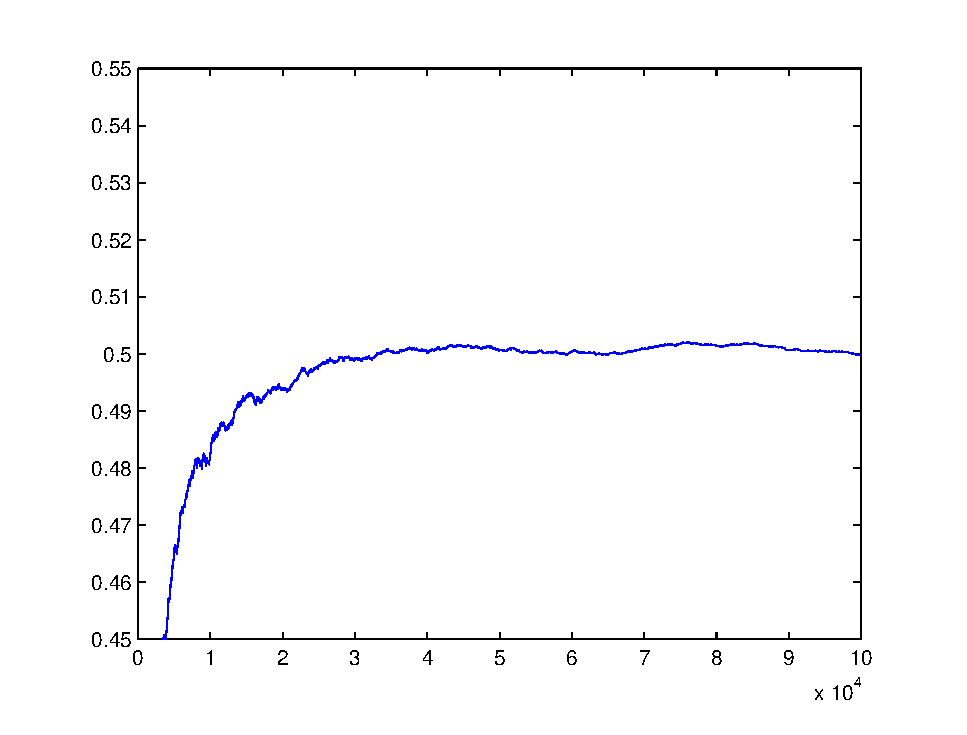
\includegraphics[scale=0.34]{images/Sensitivity_oldci_ll.eps}
} \hspace{0.5cm}
\subfigure[Old CI(XORshift, XORshift)]{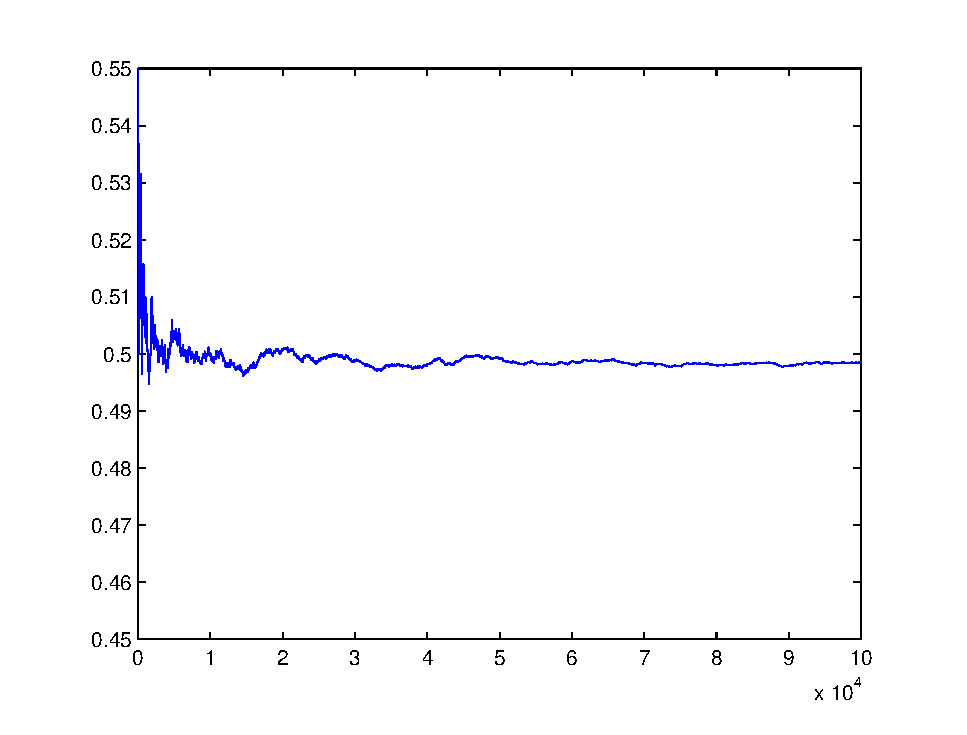
\includegraphics[scale=0.34]{images/Sensitivity_oldci_xx.eps}
} \hspace{0.5cm}
\subfigure[Old CI(ISAAC, XORshift)]{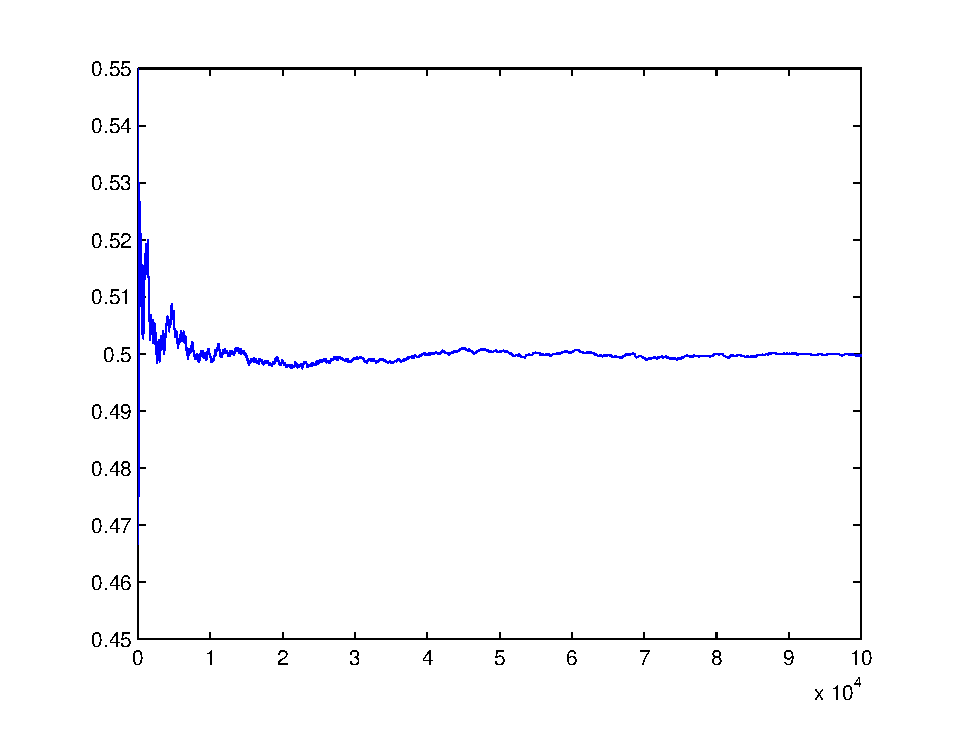
\includegraphics[scale=0.34]{images/Sensitivity_oldci_xi.eps}
} \hspace{0.5cm}
\subfigure[Old CI(ISAAC, ISAAC)]{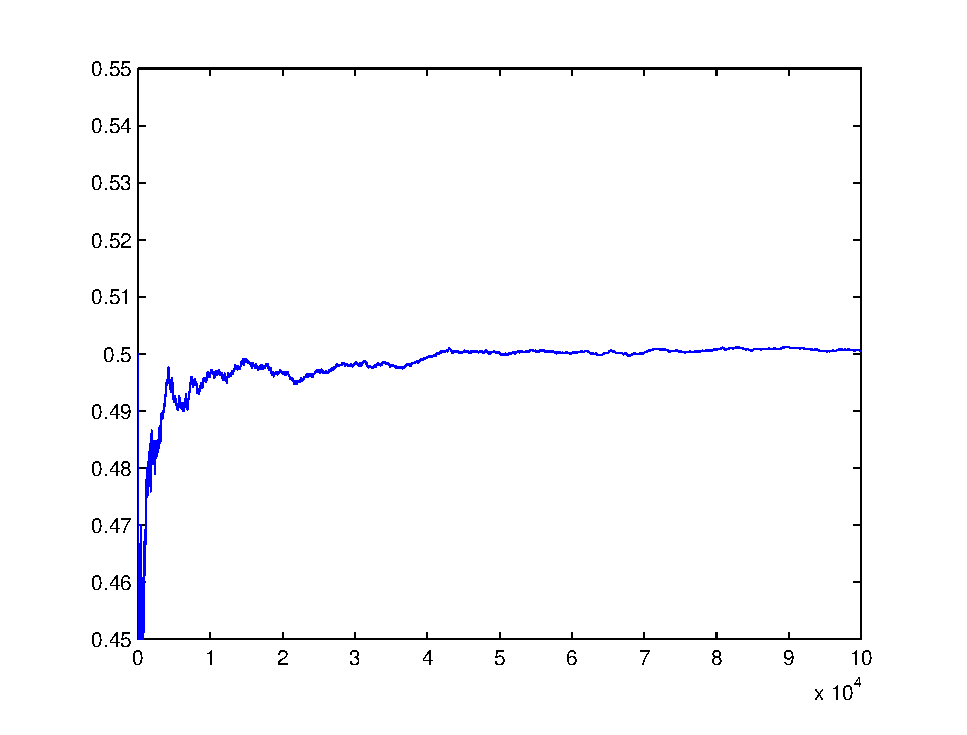
\includegraphics[scale=0.34]{images/Sensitivity_oldci_ii.eps}
} \hspace{0.5cm}
\caption{Sensitivity for old CI}
\label{Sensitivity for old CI}
\end{figure}

\begin{figure}
\centering
\subfigure[New CI(XORshift, XORshift)]{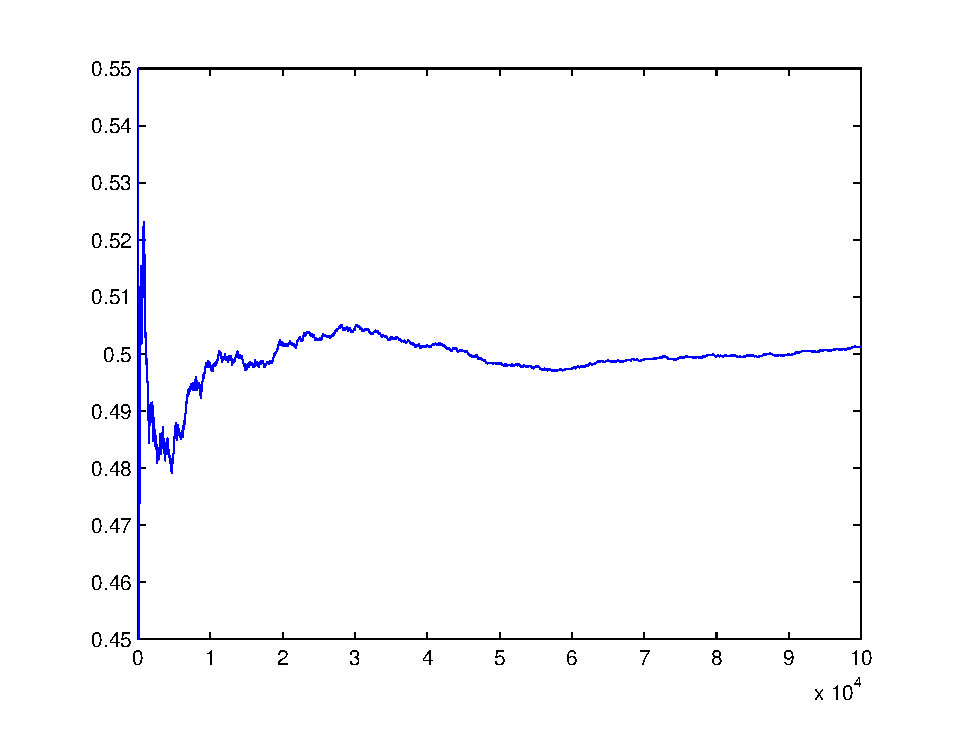
\includegraphics[scale=0.34]{images/Sensitivity_newci_xx.eps}
} \hspace{0.5cm}
\subfigure[New CI(ISAAC, XORshift)]{\includegraphics[scale=0.34]{images/Sensitivity_newci_xi.eps}
} \hspace{0.5cm}
\subfigure[New CI(ISAAC, ISAAC)]{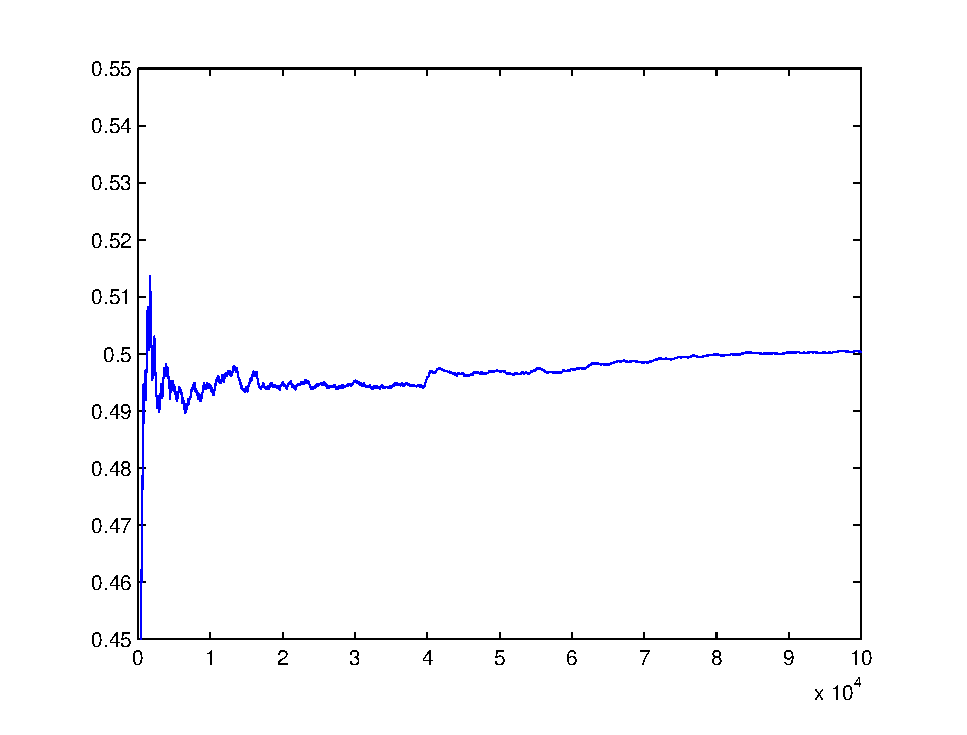
\includegraphics[scale=0.34]{images/Sensitivity_newci_ii.eps}
} \hspace{0.5cm}
\caption{Sensitivity for new CI}
\label{Sensitivity for new CI}
\end{figure}


\section{Pattern}
If a sequence consists of periodic features or repetitive patterns, it is not random [58]. These data patterns existed in the sequence can be revealed by the use of recurrence plot [59], which can be constructed as follows.

Considering a sequence ${x_0,x_1\ldots x_n}$, a vector $y_i$ of dimension $m\geqslant2$ and delay $d\geqslant1$ can be constructed by:
\begin{equation}
\centering
y_i=(x_i,x_{i+d},x_{i+2d},\ldots,x_{i+(m-1)d})
\end{equation}
The recurrence plot is then obtained by plotting a point if the following condition is satisfied:
\begin{equation}
\centering
||y_j-y_i||<t
\end{equation}
where t is a threshold distance.

Figure~\ref{The corresponding recurrence plot for old CI} and Figure~\ref{The corresponding recurrence plot for new CI} depict some sampled  recurrence plots with $m=2$, $d=1$, $t=0.05$, respectively. The points are scattered as shown in Figures, patterns can not easily observed as it is non-periodic and random.
\begin{figure}
\centering
\subfigure[Old CI(Logistic, Logistic)]{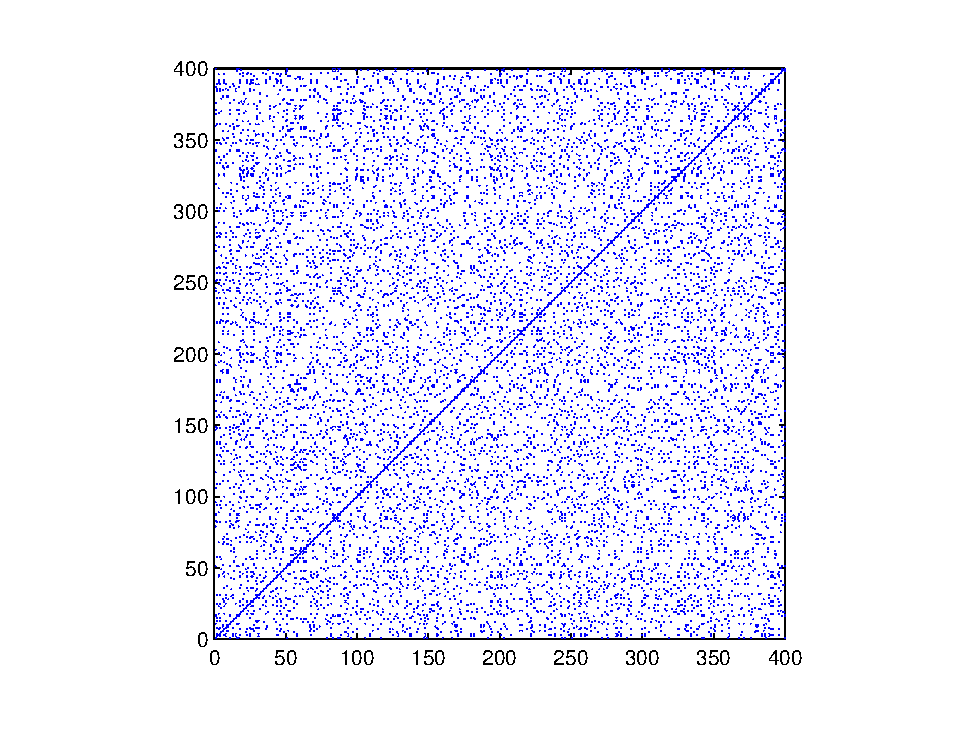
\includegraphics[scale=0.4]{images/pattern_oldci_ll.eps}
} \hspace{0.5cm}
\subfigure[Old CI(XORshift, XORshift)]{\includegraphics[scale=0.4]{images/pattern_oldci_xx.eps}
} \hspace{0.5cm}
\subfigure[Old CI(ISAAC, XORshift)]{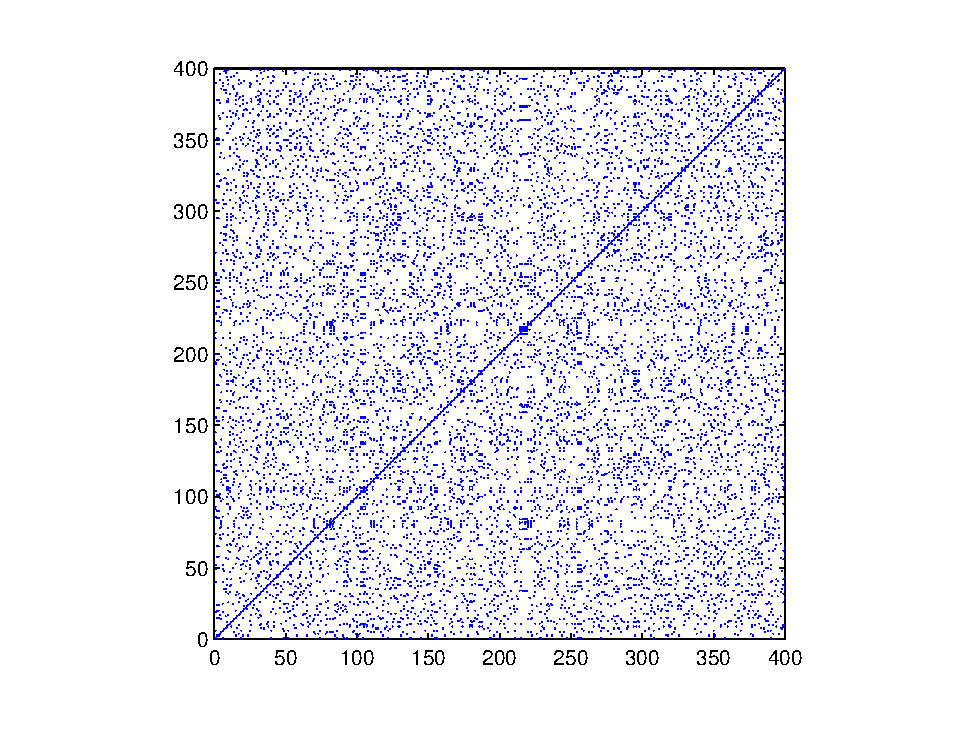
\includegraphics[scale=0.4]{images/pattern_oldci_xi.eps}
} \hspace{0.5cm}
\subfigure[Old CI(ISAAC, ISAAC)]{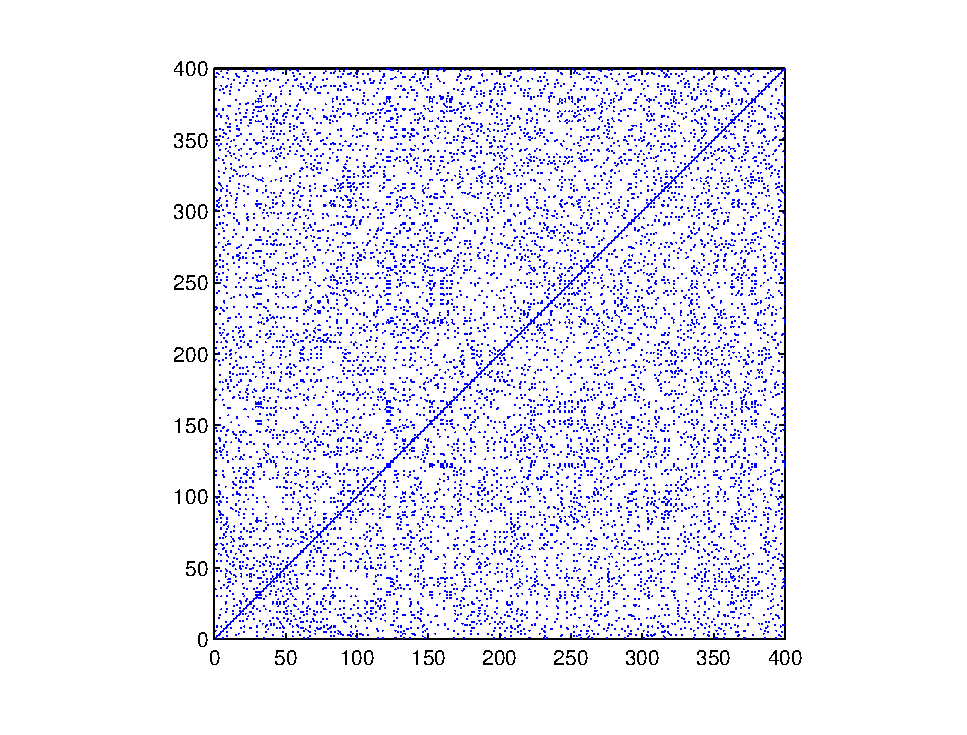
\includegraphics[scale=0.4]{images/pattern_oldci_ii.eps}
} \hspace{0.5cm}
\caption{The corresponding recurrence plot for old CI}
\label{The corresponding recurrence plot for old CI}
\end{figure}

\begin{figure}
\centering
\subfigure[New CI(XORshift, XORshift)]{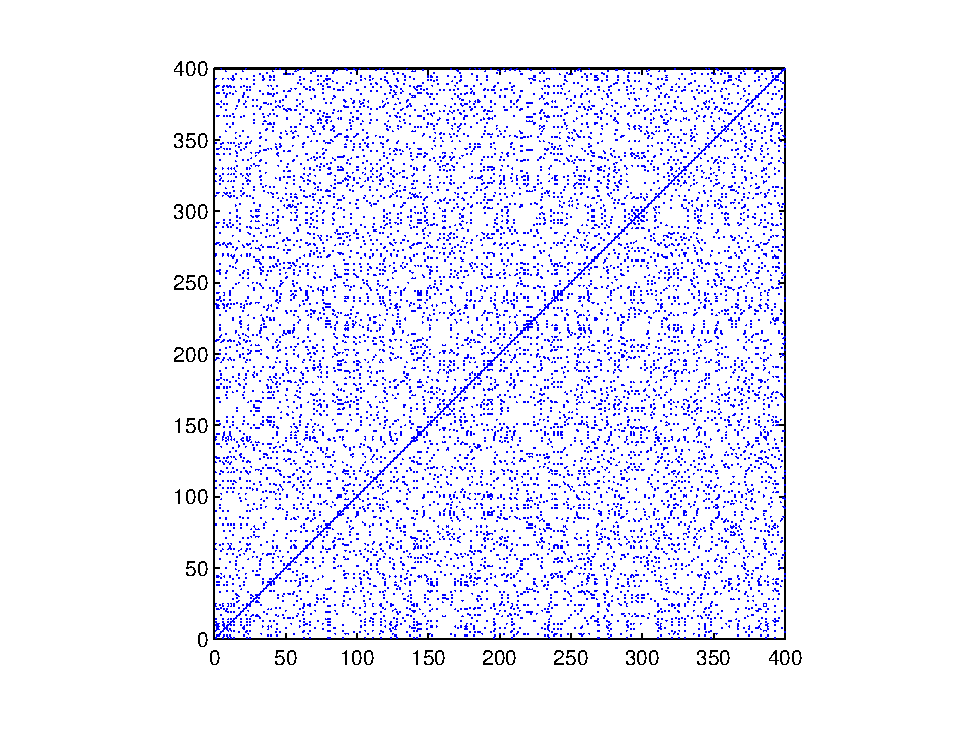
\includegraphics[scale=0.41]{images/pattern_newci_xx.eps}
} \hspace{0.5cm}
\subfigure[New CI(ISAAC, XORshift)]{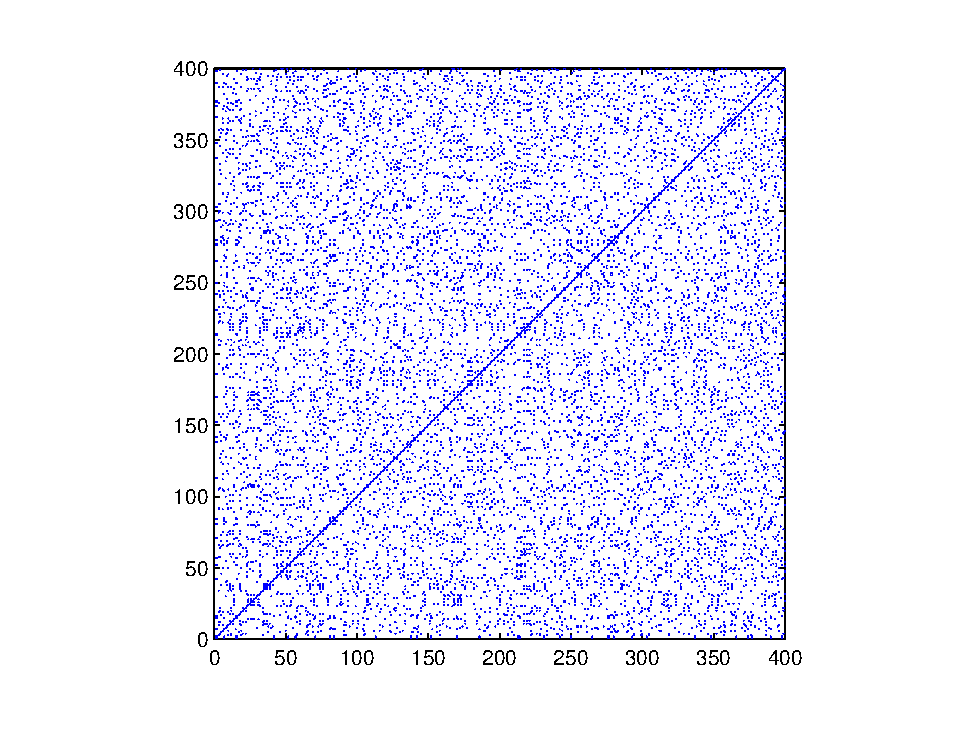
\includegraphics[scale=0.4]{images/pattern_newci_xi.eps}
} \hspace{0.5cm}
\subfigure[New CI(ISAAC, ISAAC)]{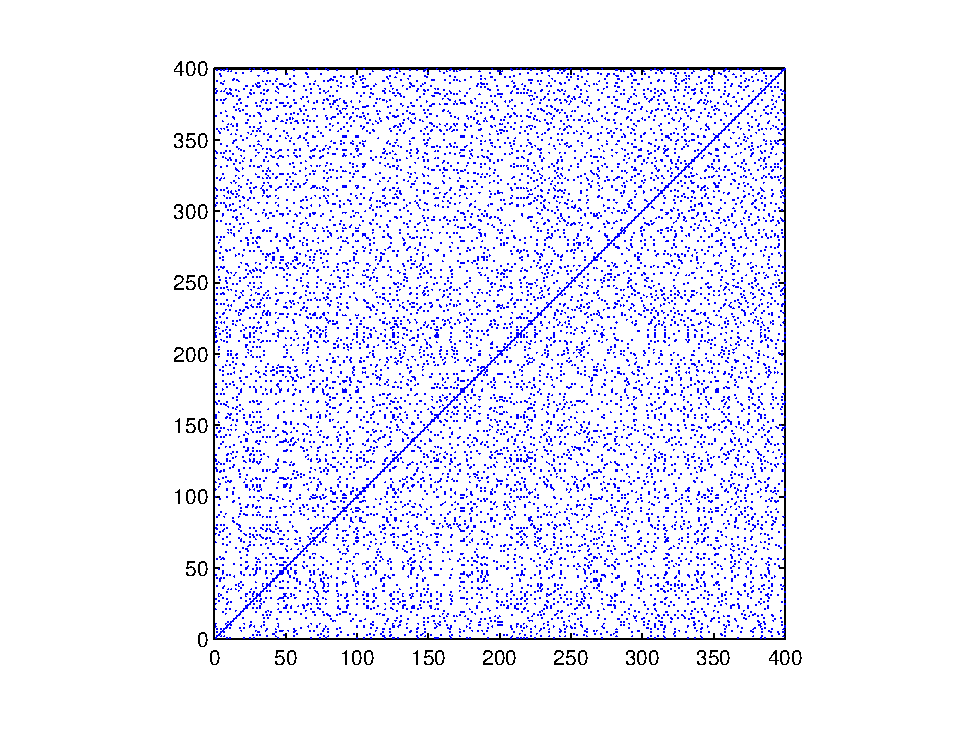
\includegraphics[scale=0.4]{images/pattern_newci_ii.eps}
} \hspace{0.5cm}
\caption{The corresponding recurrence plot for new CI}
\label{The corresponding recurrence plot for new CI}
\end{figure}


\section{Linear complexity}
A sequence is considered to be random only if it cannot be
reconstructed with a short program, or cannot be described by some simple laws. Therefore, if
a sequence is random, it has maximal complexity [60], and data compression is nearly
impossible.

The linear complexity (LC) of a sequence is the size in bits of the shortest linear feedback shift register (LFSR) which can produce this sequence. This value measures the difficulty of generating -- and perhaps analyzing -- a particular sequence.
Indeed, the randomness of a given sequence can be linked to the size of the smallest program that can produce it. LC is the size required by a LFSR to be able to produce the given sequence. The Berlekamp-Massey algorithm can measure this LC, which might be used to evaluate the ``security'' of a pseudo-random sequence.

It can be seen in Figure~\ref{Linear complexity for old CI} and Figure~\ref{Linear complexity for new CI} that the LC curves of sample sequences of 2000 b are close to the ideal line $C_i=i/2$, which imply that the generator has high linear complexity. 
\begin{figure}
\centering
\subfigure[Old CI(Logistic, Logistic)]{\includegraphics[scale=0.34]{images/linear_complexity_oldci_ll.eps}
} \hspace{0.5cm}
\subfigure[Old CI(XORshift, XORshift)]{\includegraphics[scale=0.34]{images/linear_complexity_oldci_xx.eps}
} \hspace{0.5cm}
\subfigure[Old CI(ISAAC, XORshift)]{\includegraphics[scale=0.34]{images/linear_complexity_oldci_xi.eps}
} \hspace{0.5cm}
\subfigure[Old CI(ISAAC, ISAAC)]{\includegraphics[scale=0.34]{images/linear_complexity_oldci_ii.eps}
} \hspace{0.5cm}
\caption{Linear complexity for old CI}
\label{Linear complexity for old CI}
\end{figure}

\begin{figure}
\centering
\subfigure[New CI(XORshift, XORshift)]{\includegraphics[scale=0.34]{images/linear_complexity_newci_xx.eps}
} \hspace{0.5cm}
\subfigure[New CI(ISAAC, XORshift)]{\includegraphics[scale=0.34]{images/linear_complexity_newci_xi.eps}
} \hspace{0.5cm}
\subfigure[New CI(ISAAC, ISAAC)]{\includegraphics[scale=0.34]{images/linear_complexity_newci_ii.eps}
} \hspace{0.5cm}
\caption{Linear complexity for new CI}
\label{Linear complexity for new CI}
\end{figure}


\section{Uniform distribution}

Figure~\ref{Second order distribution for old CI} and Figure~\ref{Second order distribution for new CI} give a 3D graphic representation of the distribution of a random sequence obtained by our generators. The point cloud presents a uniform distribution that tends to fill the complete 3D space, as expected for a random signal. To obtain this cloud, we have first changed the binary sequence to a $N$-bit integer sequence $x_1$, $x_2$, $x_3$, $x_4$... Then we have plot $\left(\frac{x_1}{2^N},\frac{x_2}{2^N},\frac{x_3}{2^N}\right), \left(\frac{x_2}{2^N},\frac{x_3}{2^N},\frac{x_4}{2^N}\right)$...

\begin{figure}
\centering
\subfigure[Old CI(Logistic, Logistic)]{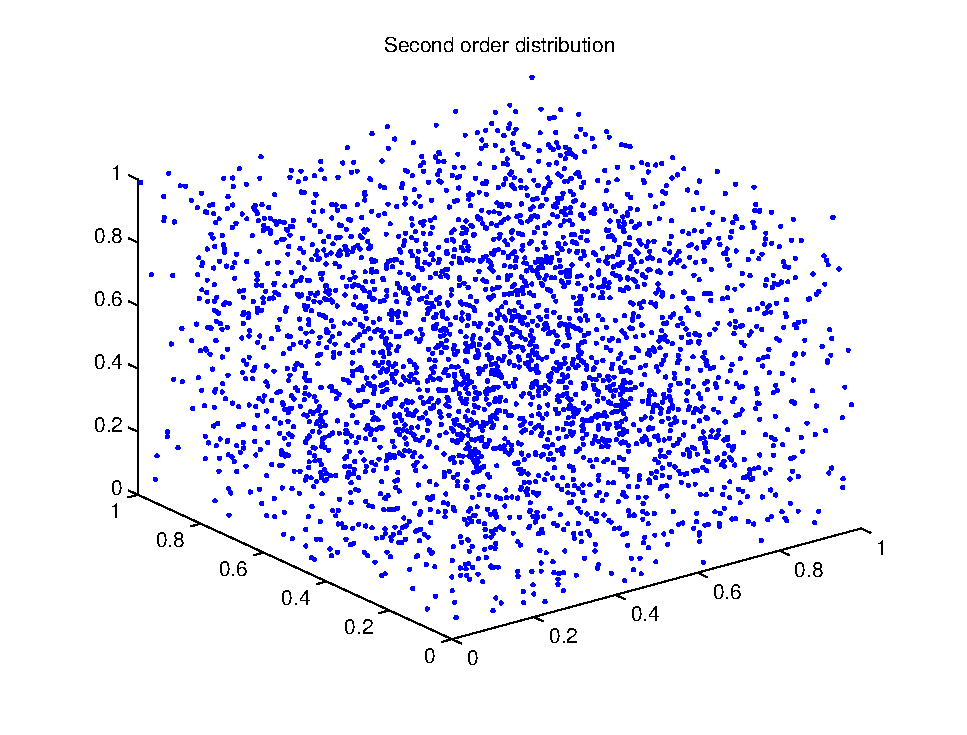
\includegraphics[scale=0.34]{images/distribution_oldci_ll.eps}
} \hspace{0.5cm}
\subfigure[Old CI(XORshift, XORshift)]{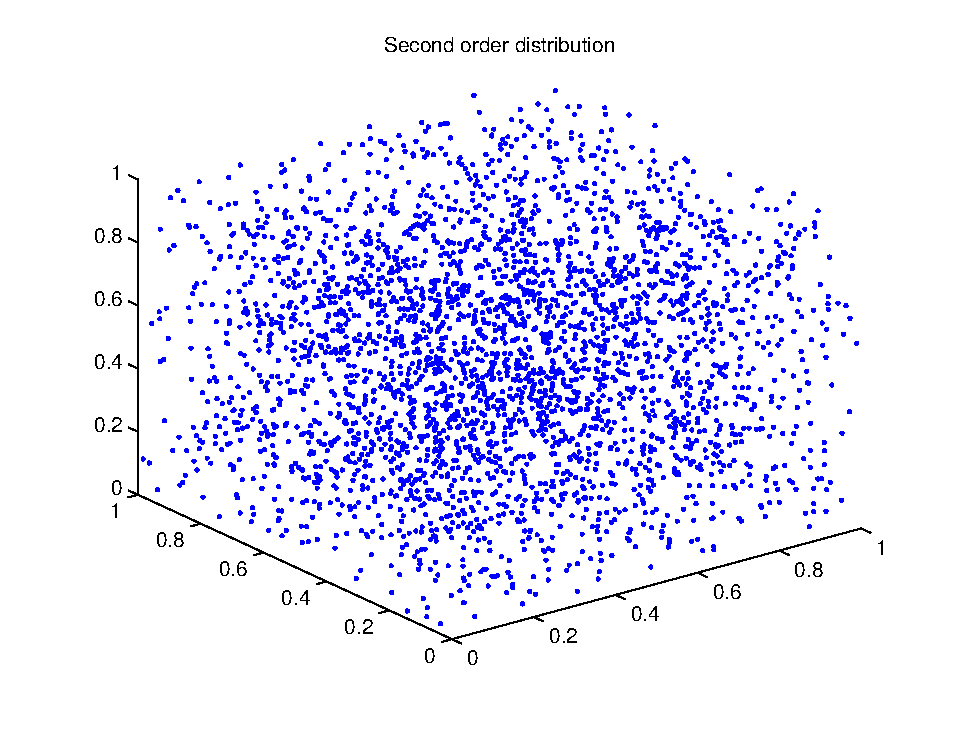
\includegraphics[scale=0.34]{images/distribution_oldci_xx.eps}
\label{Old CI(XORshift, XORshift)}} \hspace{0.5cm}
\subfigure[Old CI(ISAAC, XORshift)]{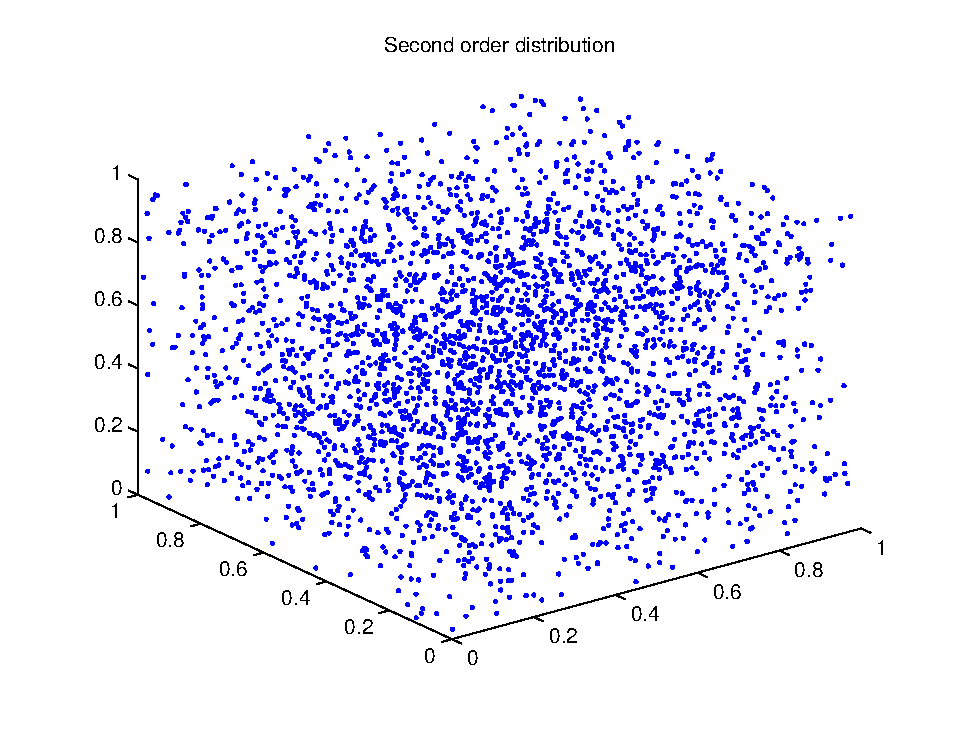
\includegraphics[scale=0.34]{images/distribution_oldci_xi.eps}
\label{Old CI(ISAAC, XORshift)}} \hspace{0.5cm}
\subfigure[Old CI(ISAAC, ISAAC)]{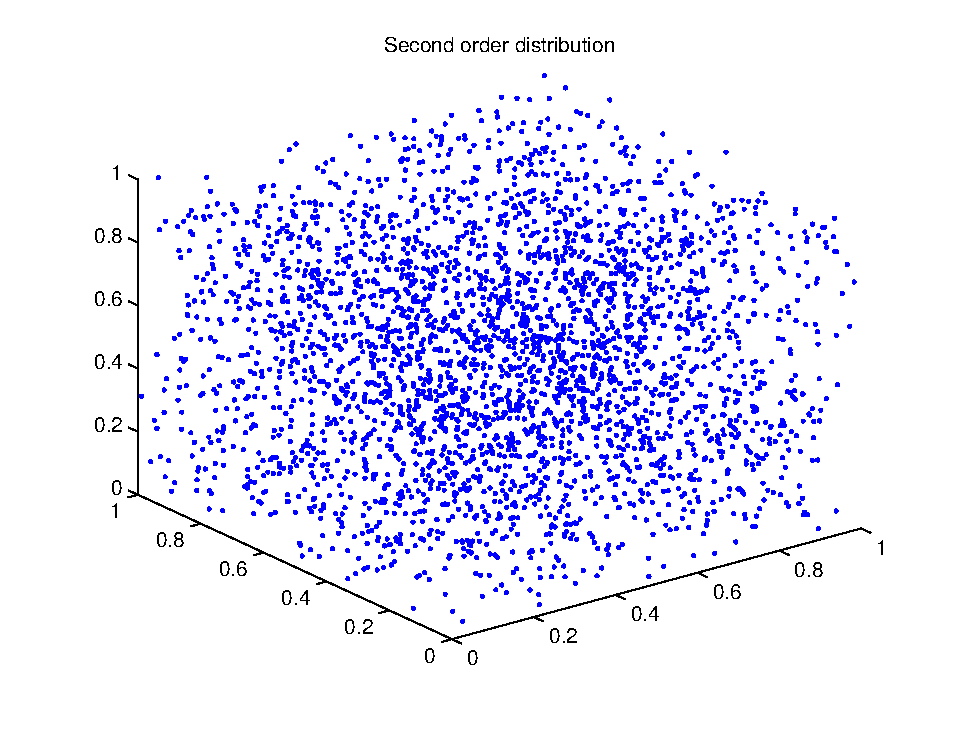
\includegraphics[scale=0.34]{images/distribution_oldci_ii.eps}
\label{Old CI(ISAAC, ISAAC)}} \hspace{0.5cm}
\caption{Second order distribution for old CI}
\label{Second order distribution for old CI}
\end{figure}

\begin{figure}
\centering
\subfigure[New CI(XORshift, XORshift)]{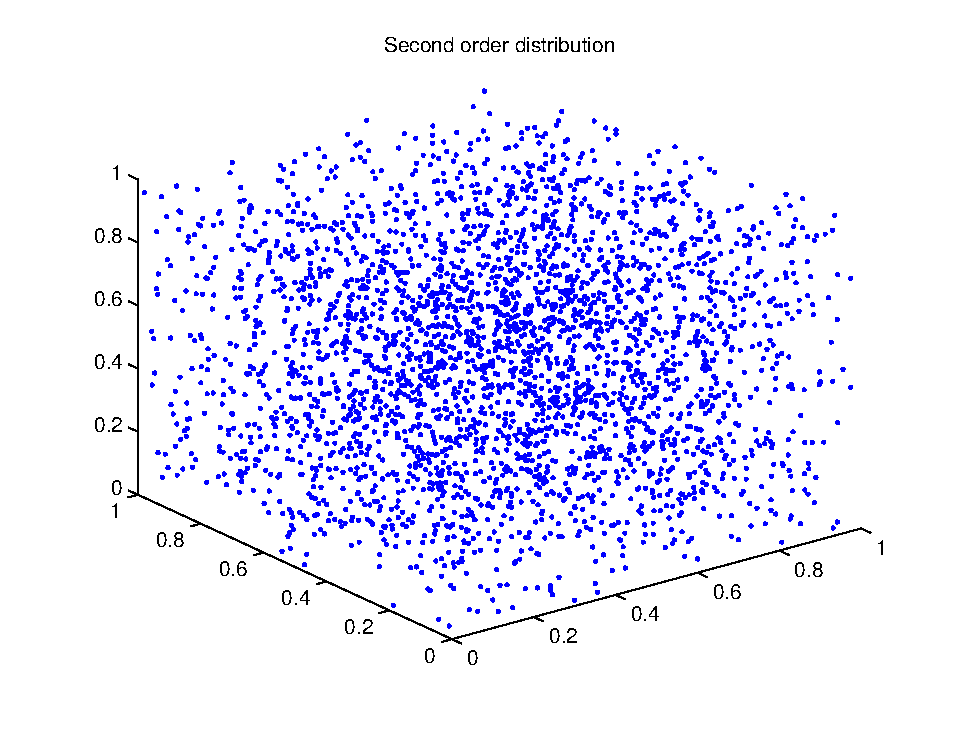
\includegraphics[scale=0.34]{images/distribution_newci_xx.eps}
} \hspace{0.5cm}
\subfigure[New CI(ISAAC, XORshift)]{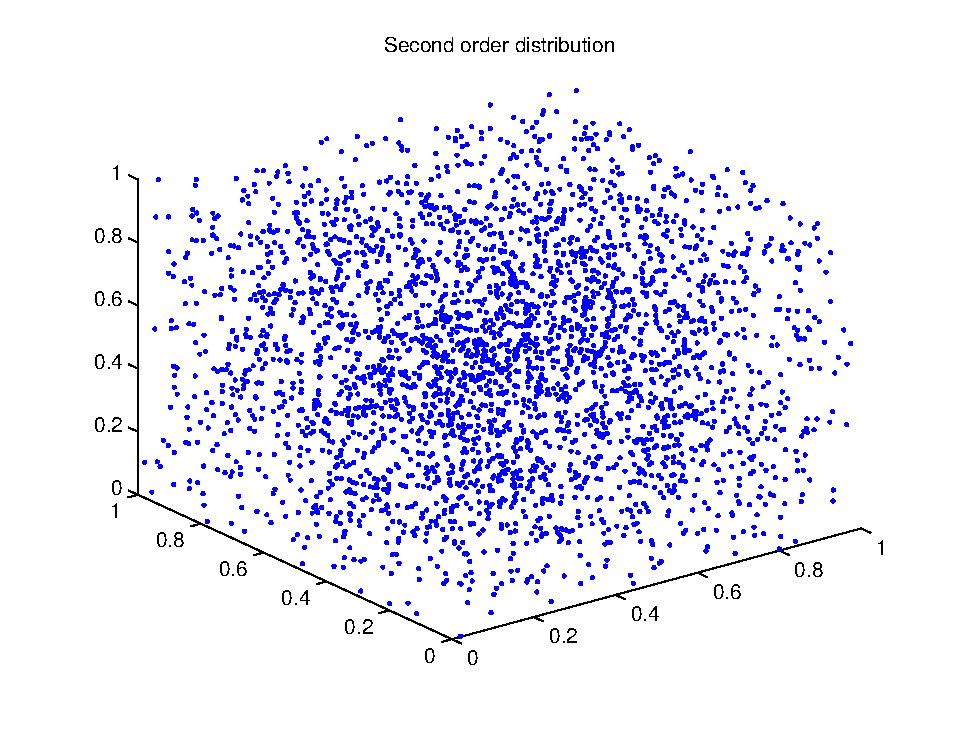
\includegraphics[scale=0.34]{images/distribution_newci_xi.eps}
} \hspace{0.5cm}
\subfigure[New CI(ISAAC, ISAAC)]{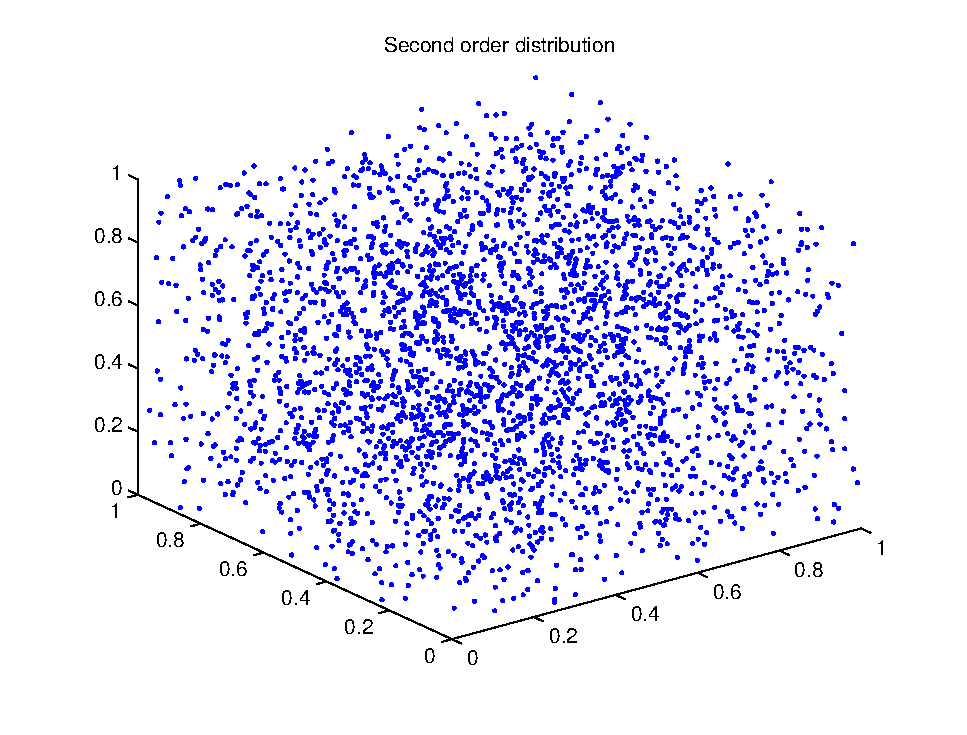
\includegraphics[scale=0.34]{images/distribution_newci_ii.eps}
} \hspace{0.5cm}
\caption{Second order distribution for new CI}
\label{Second order distribution for new CI}
\end{figure}


\section{Auto-correlation and cross-correlation}
Since the number in a random sequence should be unpredictable and hence uncorrelated,
the auto-correlation and the cross-correlation between sequences can also be used to reflect
the randomness of a sequence. These correlation values are also the prime indices when a
random sequence is to be used in spread-spectrum communications [57].

Let $\{u\}$ and $\{v\}$ be two binary $(-1,+1)$-value sequences of length $n$, the aperiodic
auto-correlation function $C_{uu}(l)$ and the aperiodic cross-correlation function $C_{uv}(l)$ are defined
in Equation (\ref{auto}) and (\ref{cross}), respectively.
\begin{equation}
\label{auto}
C_{u,u}(l)=
\left\{
\begin{array}{llc}
\sum_{i=0}^{n-1-l} u_{i}u_{i+l} & \text{ if }&0\leqslant l\leqslant n-1\\
\sum_{i=0}^{n-1+l} u_{i-l}u_{i}  & \text{ if }&1-n\leqslant l\leqslant 0 \\
0 & \text{ if }&|l|\geqslant n\\
\end{array}
\right.
\end{equation}
\begin{equation}
\label{cross}
C_{u,v}(l)=
\left\{
\begin{array}{llc}
\sum_{i=0}^{n-1-l} u_{i}v_{i+l} & \text{ if }&0\leqslant l\leqslant n-1\\
\sum_{i=0}^{n-1+l} u_{i-l}v_{i}  & \text{ if }&1-n\leqslant l\leqslant 0 \\
0 & \text{ if }&|l|\geqslant n\\
\end{array}
\right.
\end{equation}


The auto-correlation and cross-correlation of the symbolic sequences are respectively given in Figure.~\ref{autocorr for old CI}, Figure.~\ref{autocorr for new CI}, Figure.~\ref{intercorr for old CI} and Figure.~\ref{intercorr for new CI}demonstrating a nice nature. It can be seen that this sequences have $\delta$-like auto-correlation which is required for a good PRBNG. The sequences generated with different initial values will have zero cross-correlation due to the sensitive dependence on initial conditions. 



\begin{figure}
\centering
\subfigure[Old CI(Logistic, Logistic)]{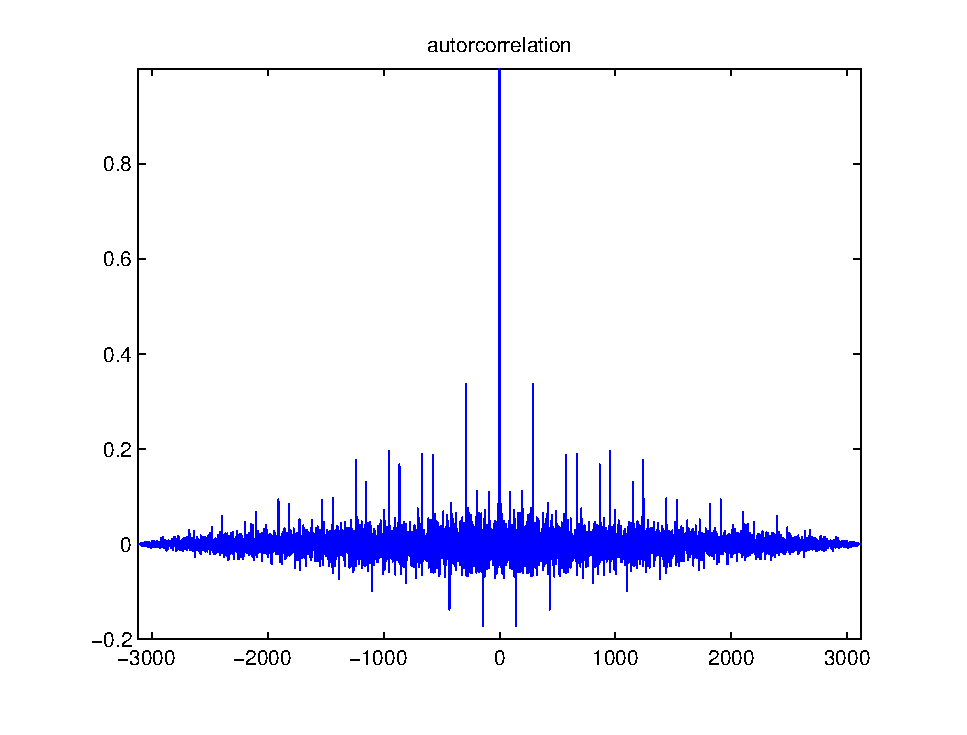
\includegraphics[scale=0.34]{images/autocorr_oldci_ll.eps}
} \hspace{0.5cm}
\subfigure[Old CI(XORshift, XORshift)]{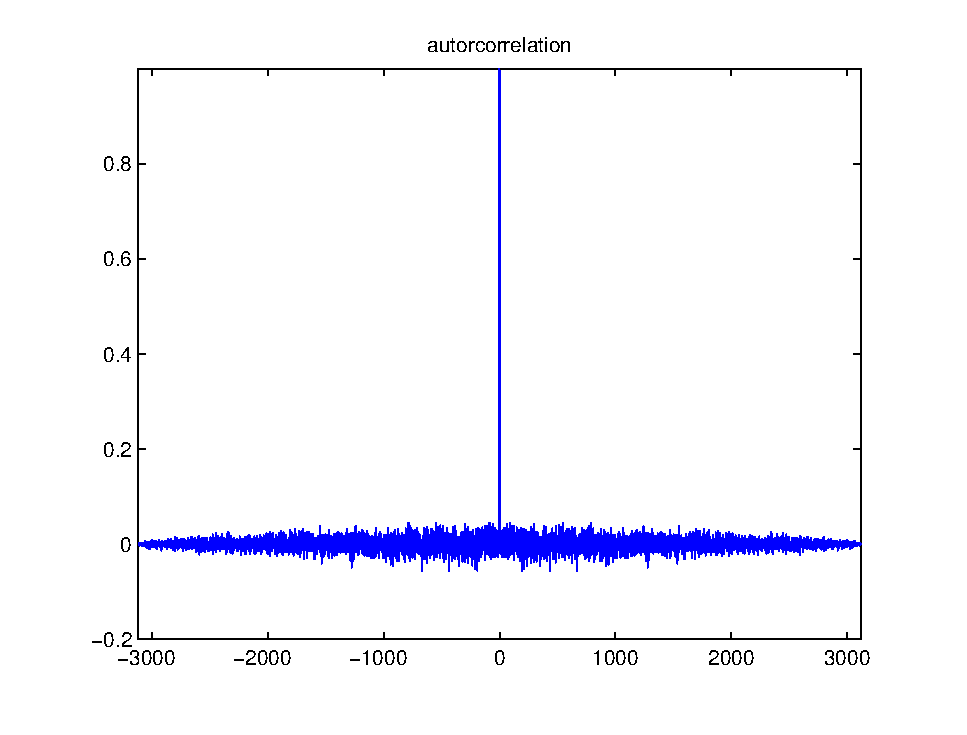
\includegraphics[scale=0.34]{images/autocorr_oldci_xx.eps}
} \hspace{0.5cm}
\subfigure[Old CI(ISAAC, XORshift)]{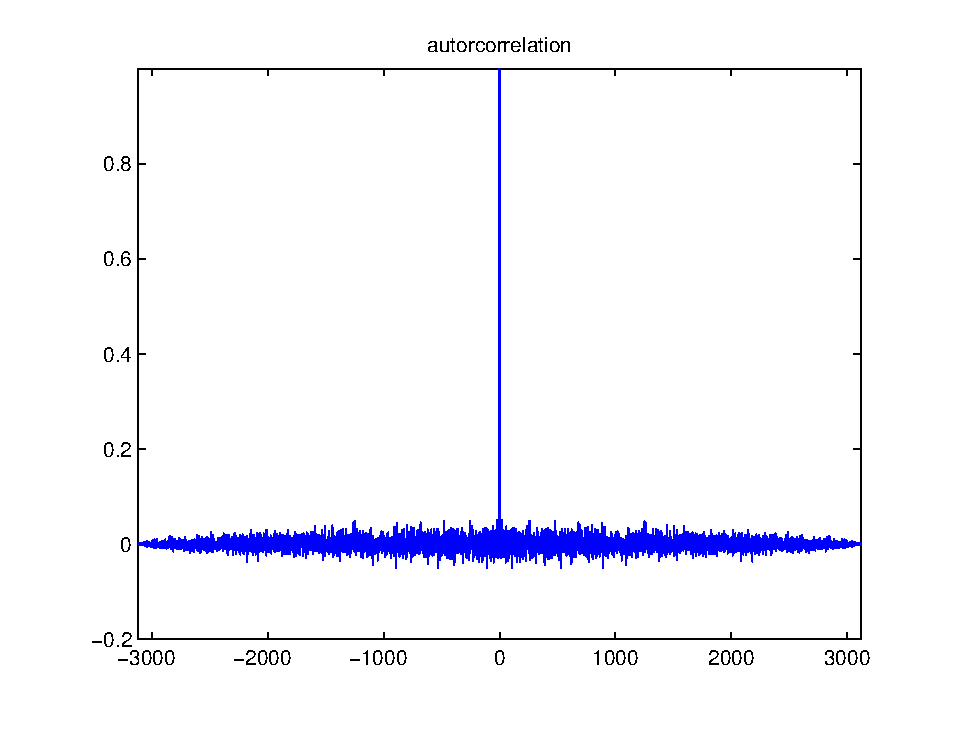
\includegraphics[scale=0.34]{images/autocorr_oldci_xi.eps}
} \hspace{0.5cm}
\subfigure[Old CI(ISAAC, ISAAC)]{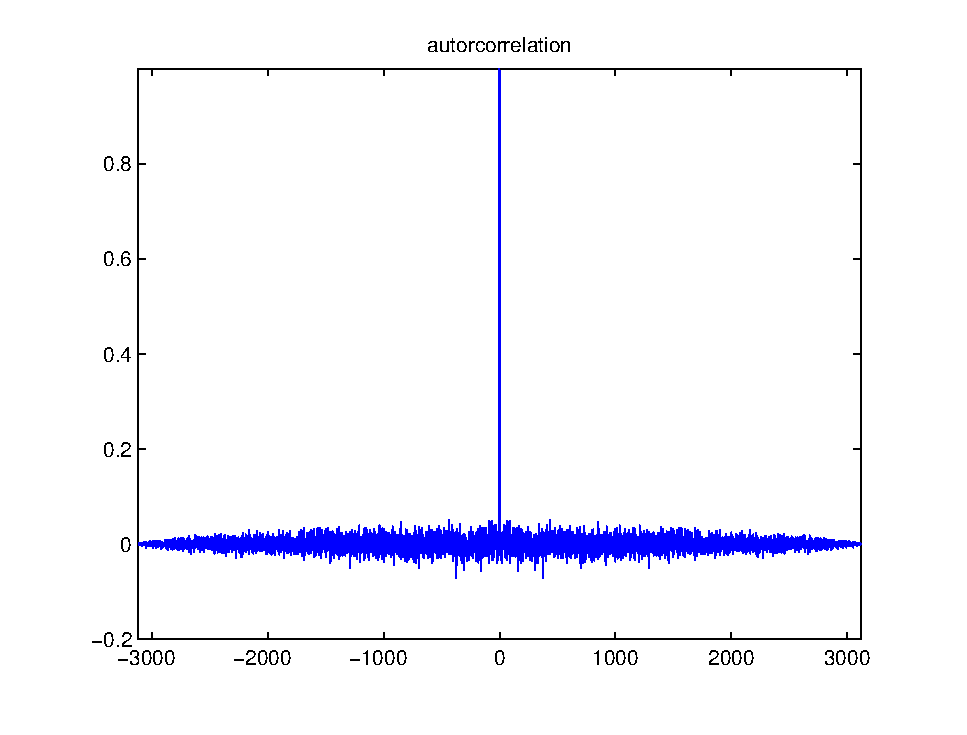
\includegraphics[scale=0.34]{images/autocorr_oldci_ii.eps}
} \hspace{0.5cm}
\caption{Auto-correlation for old CI}
\label{autocorr for old CI}
\end{figure}

\begin{figure}
\centering
\subfigure[New CI(XORshift, XORshift)]{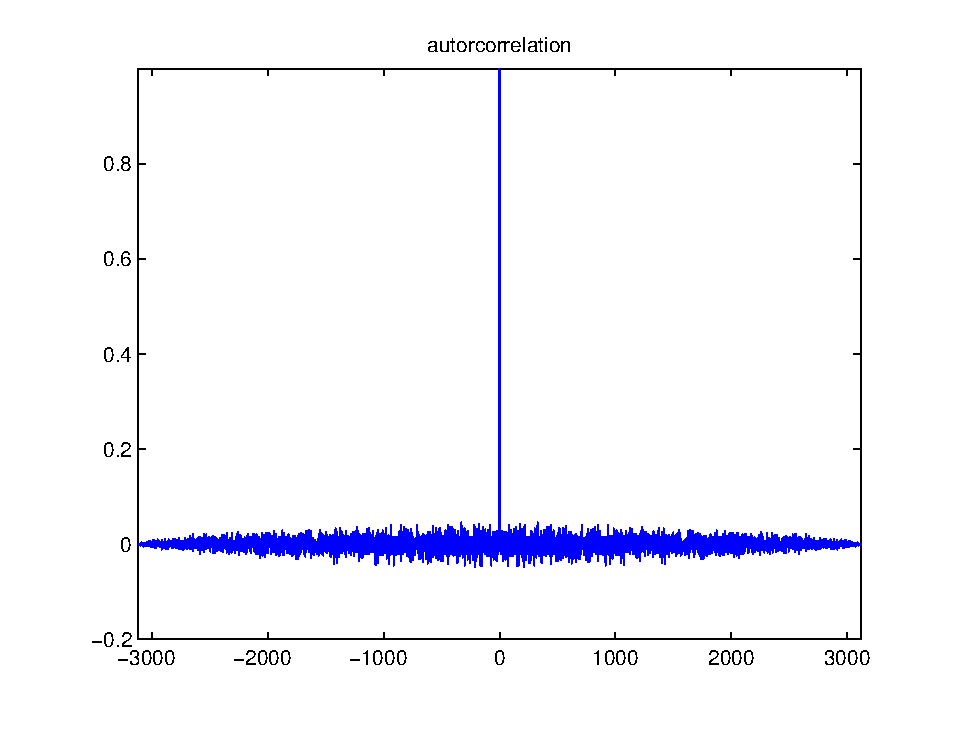
\includegraphics[scale=0.34]{images/autocorr_newci_xx.eps}
} \hspace{0.5cm}
\subfigure[New CI(ISAAC, XORshift)]{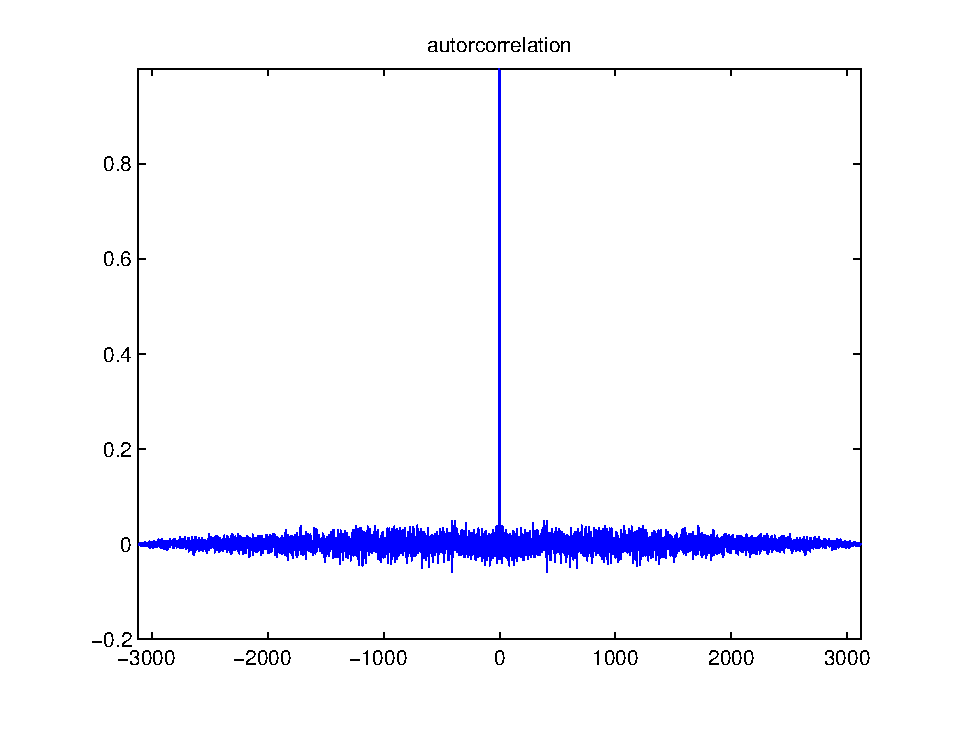
\includegraphics[scale=0.34]{images/autocorr_newci_xi.eps}
} \hspace{0.5cm}
\subfigure[New CI(ISAAC, ISAAC)]{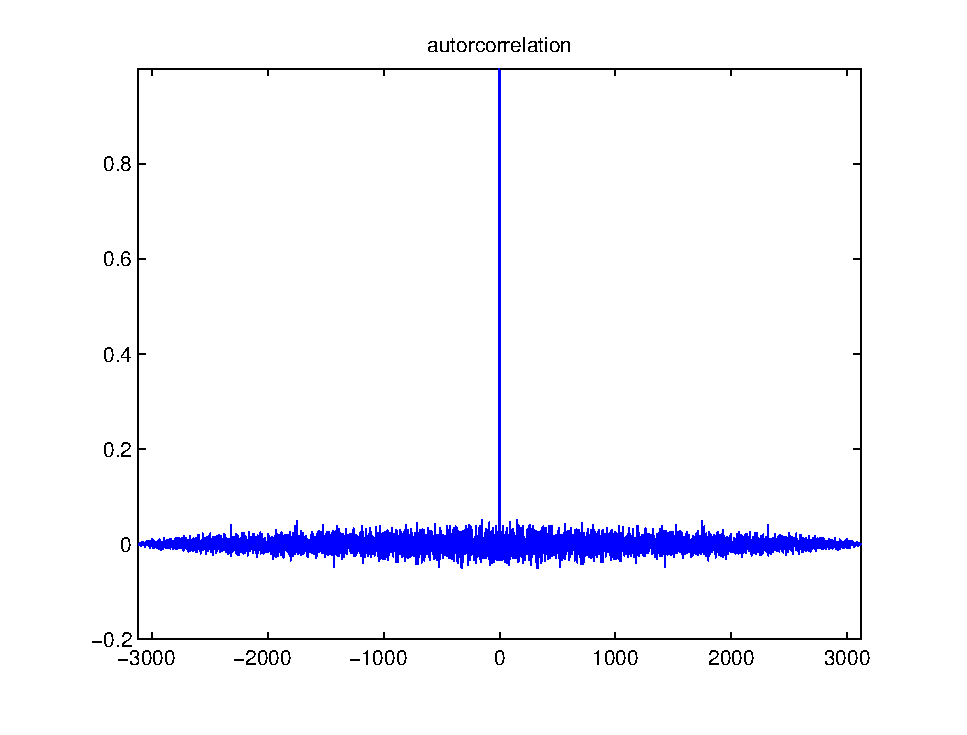
\includegraphics[scale=0.34]{images/autocorr_newci_ii.eps}
} \hspace{0.5cm}
\caption{Auto-correlation for new CI}
\label{autocorr for new CI}
\end{figure}

\begin{figure}
\centering
\subfigure[Old CI(Logistic, Logistic)]{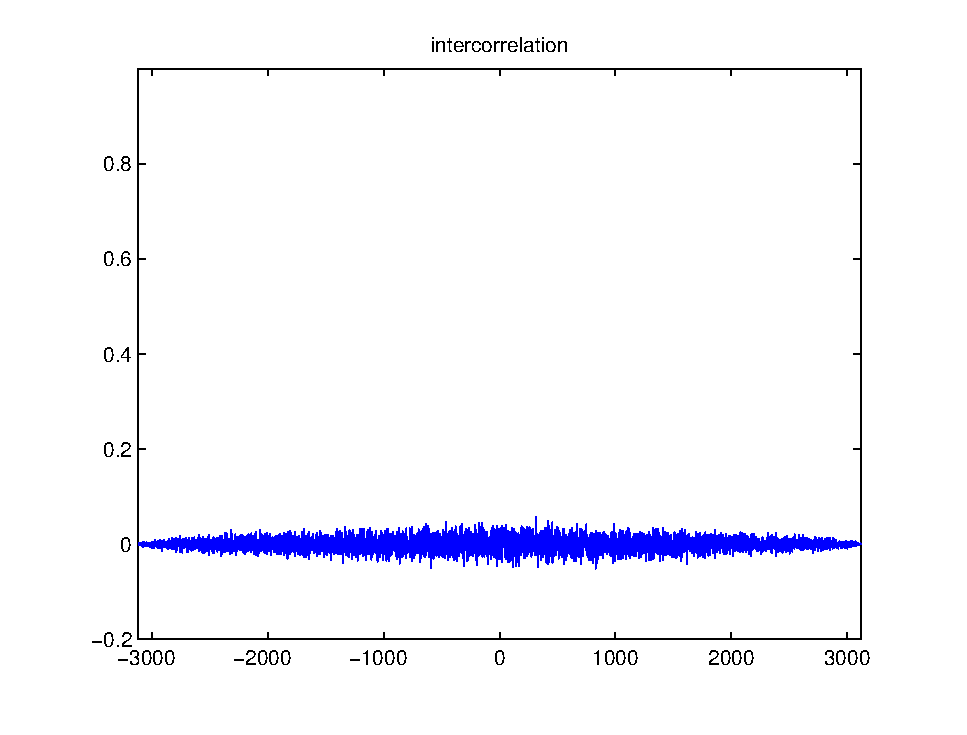
\includegraphics[scale=0.34]{images/intercorr_oldci_ll.eps}
} \hspace{0.5cm}
\subfigure[Old CI(XORshift, XORshift)]{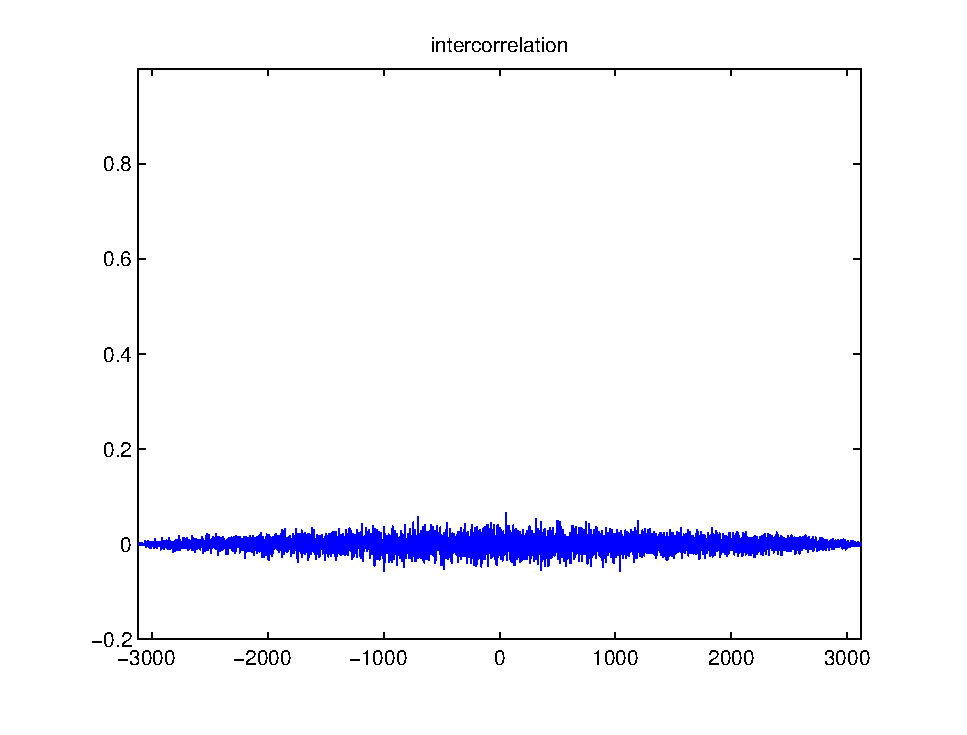
\includegraphics[scale=0.34]{images/intercorr_oldci_xx.eps}
} \hspace{0.5cm}
\subfigure[Old CI(ISAAC, XORshift)]{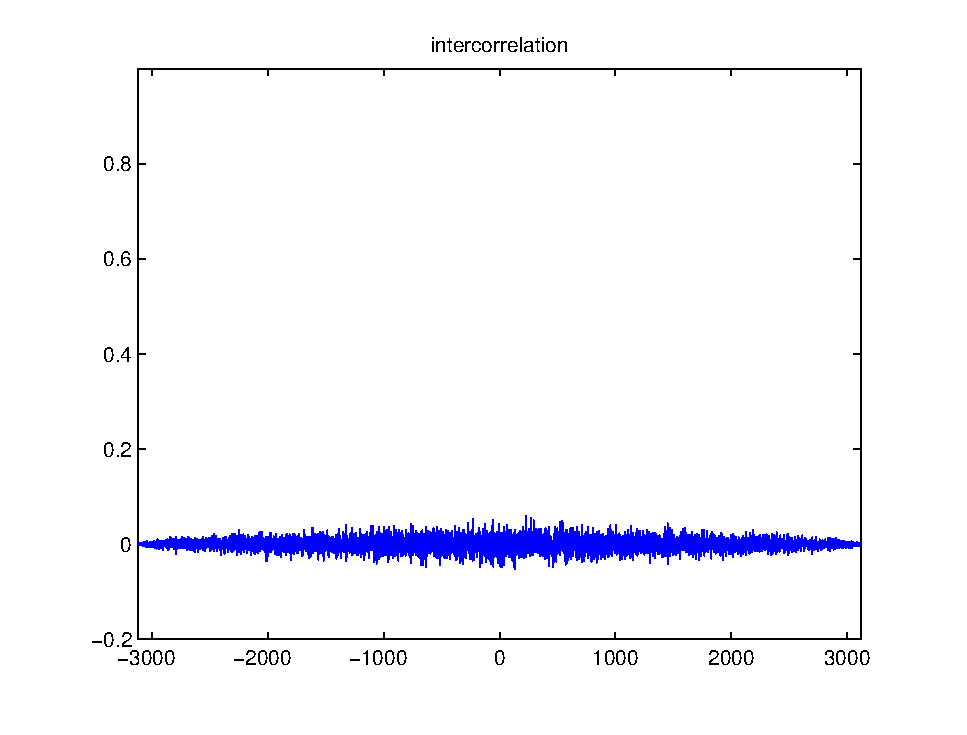
\includegraphics[scale=0.34]{images/intercorr_oldci_xi.eps}
} \hspace{0.5cm}
\subfigure[Old CI(ISAAC, ISAAC)]{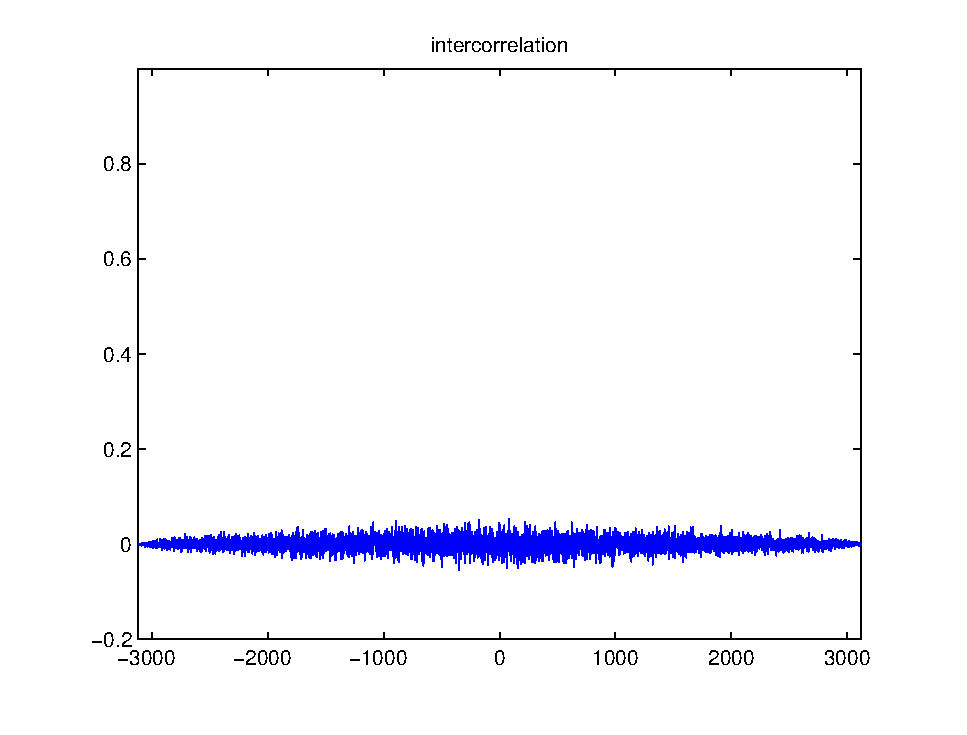
\includegraphics[scale=0.34]{images/intercorr_newci_ii.eps}
} \hspace{0.5cm}
\caption{Cross-correlation for old CI}
\label{intercorr for old CI}
\end{figure}

\begin{figure}
\centering
\subfigure[New CI(XORshift, XORshift)]{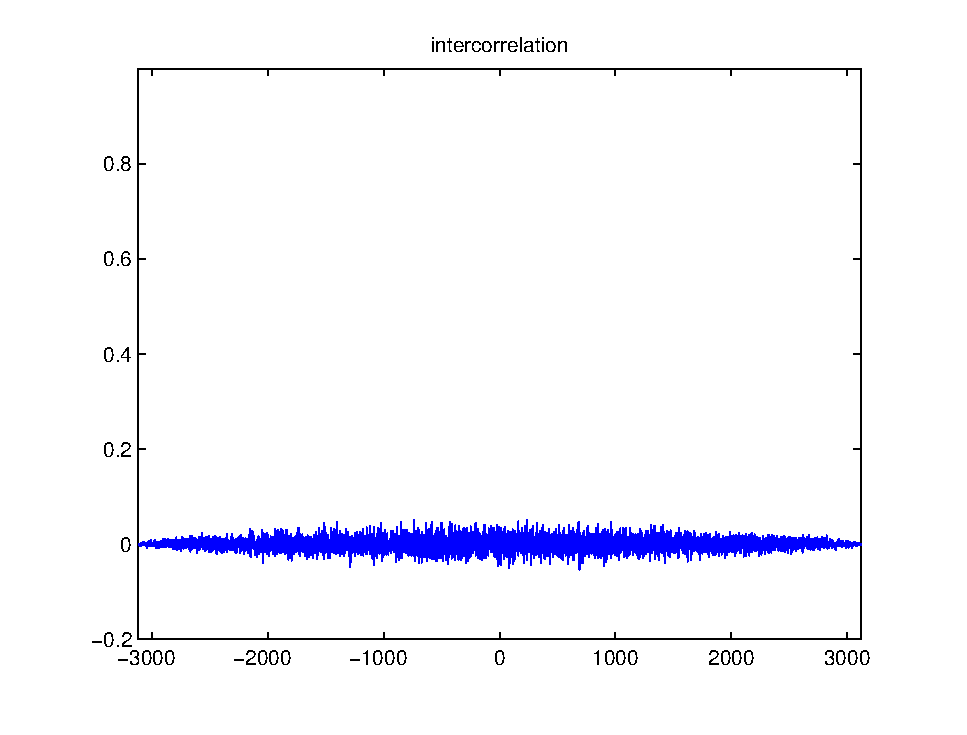
\includegraphics[scale=0.34]{images/intercorr_newci_xx.eps}
} \hspace{0.5cm}
\subfigure[New CI(ISAAC, XORshift)]{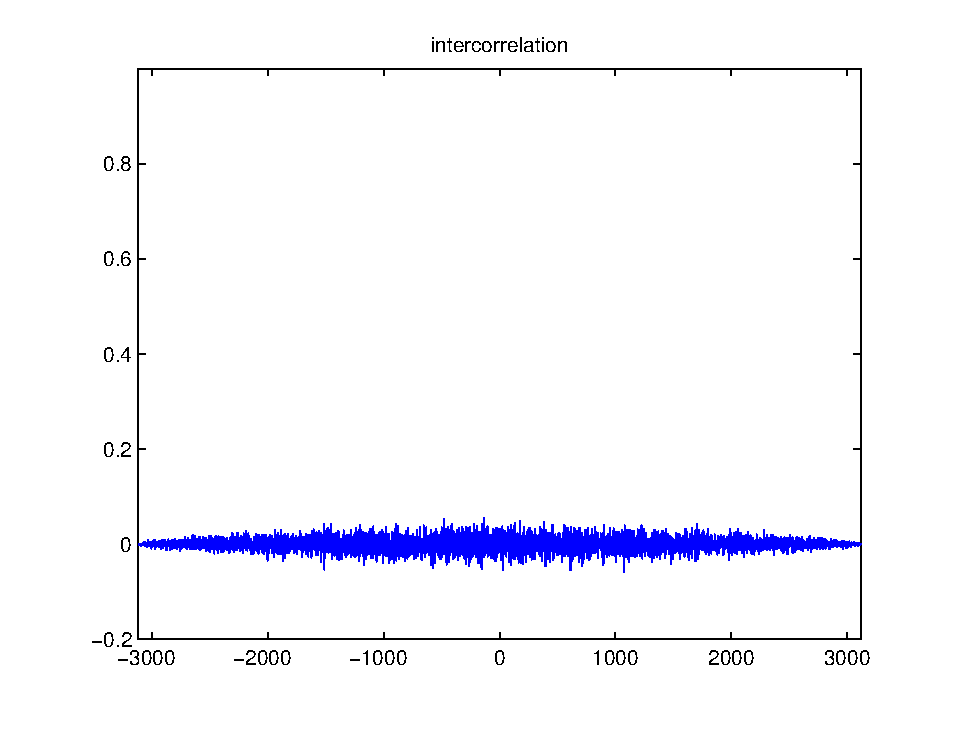
\includegraphics[scale=0.34]{images/intercorr_newci_xi.eps}
} \hspace{0.5cm}
\subfigure[New CI(ISAAC, ISAAC)]{\includegraphics[scale=0.34]{images/intercorr_newci_ii.eps}
} \hspace{0.5cm}
\caption{Cross-correlation for new CI}
\label{intercorr for new CI}
\end{figure}
\section{FFT}

The FFT of the sequences (Figure.~\ref{FFT for old CI} and Figure.~\ref{FFT for new CI}) are performed and the corresponding power spectrums are computed. Some complete flat power spectrums, with almost equal frequency contribution for all frequencies, are indicative of a total random series.

\begin{figure}
\centering
\subfigure[Old CI(Logistic, Logistic)]{\includegraphics[scale=0.34]{images/fft_oldci_ll.eps}
} \hspace{0.5cm}
\subfigure[Old CI(XORshift, XORshift)]{\includegraphics[scale=0.34]{images/fft_oldci_xx.eps}
} \hspace{0.5cm}
\subfigure[Old CI(ISAAC, XORshift)]{\includegraphics[scale=0.34]{images/fft_oldci_xi.eps}
} \hspace{0.5cm}
\subfigure[Old CI(ISAAC, ISAAC)]{\includegraphics[scale=0.34]{images/fft_oldci_ii.eps}
} \hspace{0.5cm}
\caption{FFT for old CI}
\label{FFT for old CI}
\end{figure}

\begin{figure}
\centering
\subfigure[New CI(XORshift, XORshift)]{\includegraphics[scale=0.34]{images/fft_newci_xx.eps}
} \hspace{0.5cm}
\subfigure[New CI(ISAAC, XORshift)]{\includegraphics[scale=0.34]{images/fft_newci_xi.eps}
} \hspace{0.5cm}
\subfigure[New CI(ISAAC, ISAAC)]{\includegraphics[scale=0.34]{images/fft_newci_ii.eps}
} \hspace{0.5cm}
\caption{FFT for new CI}
\label{FFT for new CI}
\end{figure}

\section{Devaney's Chaos Property}

Generally speaking, the quality of a PRNG depends, to a large extent, on the following criteria: randomness, uniformity, independence, storage efficiency, and reproducibility. A chaotic sequence may satisfy these requirements and also other chaotic properties, as ergodicity, entropy, and expansivity. A chaotic sequence is extremely sensitive to the initial conditions. That is, even a minute difference in the initial state of the system can lead to enormous differences in the final state, even over fairly small timescales. Therefore, chaotic sequence fits the requirements of pseudo-random sequence well. Contrary to XORshift and ISAAC, our generator possesses these chaotic properties~\cite{guyeux09},\cite{wang2009}.
However, despite a large number of papers published in the field of chaos-based pseudo-random generators, the impact of this research is rather marginal. This is due to the following reasons: almost all PRNG algorithms using chaos are based on dynamical systems defined on continuous sets (\emph{e.g.}, the set of real numbers). So these generators are usually slow, requiring considerably more storage space, and lose their chaotic properties during computations as mentioned earlier in this paper. These major problems restrict their use as generators~\cite{Kocarev2001}.

In this paper we do not simply integrate chaotic maps hoping that the implemented algorithm remains chaotic. Indeed, the PRNGs we conceive are just discrete chaotic iterations and we have proven in \cite{guyeux09} that these iterations produce a topological chaos as defined by Devaney: they are regular, transitive, and sensitive to initial conditions. This famous definition of a chaotic behavior for a dynamical system implies unpredictability, mixture, sensitivity, and uniform repartition. Moreover, as only integers are manipulated in discrete chaotic iterations, the chaotic behavior of the system is preserved during computations, and these computations are fast.

Let us now explore the topological properties of our generator and their consequences concerning the quality of the generated pseudo-random sequences.
%Generally speaking, the success of a PRNG study depends, to a large extent, on the following criteria:
%uniformity, independence, storage efficiency, reproducibility. Chaotic sequence
%has not only these good pseudo-random characteristics but also chaotic properties,
%as ergodicity, entropy and expansivity. It is extremely sensitive to the initial states. That is, even a minute
%difference in the starting state of the
%system can lead to enormous differences in the final state of the system even over
%fairly small timescales. Therefore, chaotic sequence well fits the requirements of
%pseudo-random sequence.\newline
%Despite a huge number of papers published in the field of chaos-based pseudo-random generators, the impact that this research has made on conventional cryptography is rather marginal. This is due to the following reasons: almost all chaotic algorithms are based on dynamical systems defined on the set of real numbers. So these generators are usually slow, require considerably more storage space and lose their chaotic property during computations. These major problems restrict their use in cryptography~\cite{Kocarev2001}.\newline
%The generator proposed in this paper does not inherit its chaotic properties from a real chaotic map, but from chaotic iterations defined in Section \ref{subsection:Chaotic iterations}. It has been proved in~\cite{guyeux09} that chaotic iterations behave as chaos, as it is defined by Devaney: they are regular, transitive and sensitive to initial conditions. This most famous definition of a chaotic behavior for a dynamical system implies unpredictability, mixture, sensitivity
%and uniform repartition. The principal interest is that chaotic iterations don't use real numbers.
%This allows the creation of a new generation of chaotic pseudo-random number generators. Because only integers are manipulated in chaotic iterations, the chaotic behavior of the system is preserved during computations, and these computations are fast.


\section{Topological Consequences}

We have proven in \cite{gfb10:ip} that chaotic iterations are expansive and topologically mixing. These topological properties are inherited by the generators we presented here. In particular, any error on the seed are magnified until being equal to the constant of expansivity.
We will now investigate the consequences of being chaotic, as defined by Devaney. 

First of all, the transitivity property implies the indecomposability of the system:

\begin{definition}
A dynamical system $\left( \mathcal{X}, f\right)$ is indecomposable if it is not the union of two closed sets $A, B \subset \mathcal{X}$ such that $f(A) \subset A, f(B) \subset B$.
\end{definition}

Thus it is impossible to reduce the set of the outputs generated by our PRNG, in order to reduce its complexity. Moreover, it is possible to show that Old and New CI generators are strongly transitive:

\begin{definition}
A dynamical system $\left( \mathcal{X}, f\right)$ is strongly transitive if $\forall x,y \in \mathcal{X},$ $\forall r > 0,$ $\exists z \in \mathcal{X},$ $d(z,x) \leqslant r \Rightarrow$ $\exists n \in \mathds{N}^*,$ $f^n(z)=y$.
\end{definition}

In other words, for all $x,y \in \mathcal{X}$, it is possible to find a point $z$ in the neighborhood of $x$ such that an iterate $f^n(z)$ is $y$. Indeed, this result has been established during the proof of the transitivity presented in~\cite{guyeux09}. Among other things, the strong transitivity property leads to the fact that without the knowledge of the seed, all of the outputs are possible. Additionally, no point of the output space can be discarded when studying our PRNG: it is intrinsically complicated and it cannot be simplified.

Finally, these generators possess the instability property:

\begin{definition}
A dynamical system $\left( \mathcal{X}, f\right)$ is unstable if for all $x \in \mathcal{X}$, the orbit $\gamma_x:n \in \mathds{N} \longmapsto f^n(x)$ is unstable, that is: $\exists \varepsilon > 0,$ $\forall \delta > 0,$ $\exists y \in \mathcal{X},$ $\exists n \in \mathds{N},$ $d(x,y) < \delta$ and $d\left(\gamma_x(n), \gamma_y(n)\right) \geqslant \varepsilon.$
\end{definition}

This property, which is implied by the sensitive dependence to the initial condition, leads to the fact that in all of the neighborhoods of any $x$, there are points which are separate from $x$ under iterations of $f$. We thus can claim that the behavior of our generators is unstable.




\chapter{The family of CIs PRNG}
\label{ThefamilyofCIPRNG}
\minitoc
\section{Mapping matrix}

Chaotic iterations introduced above can be described by using the mapping matrix defined bellow.

\begin{definition}
Let $f:\mathds{B}^{\mathsf{N}}\longrightarrow \mathds{B}^{\mathsf{N}}$
be an iteration function, then its associated \emph{mapping matrix}
$\mathsf{f}$ is the matrix of size $\mathsf{N} \times 2^\mathsf{N}$ whose element  $\mathsf{f}_{p,q}$ is the integer having the following binary decomposition:  $q_\mathsf{N}, \hdots, q_{\mathsf{N}-p}, f(q)_{\mathsf{N}-p+1}, q_{\mathsf{N}-p+2}, \hdots, q_1  $, where $q_i$ (resp. $f(q)_i$) is the $i-$th binary digit of $q$ (resp. of $f(q)$).
%$x_1, \hdots, x_\mathsf{N}$, where $x_i$ that is:
%\begin{itemize}
%\item $x_i$ is the $p-$th binary digit of $f(q)$, if $i=p$,
%\item the $i-$th binary digit of $q$, else.
%\end{itemize}
%$$\mathsf{f} =
%\left(
%\begin{array}{cccc}
%f(0)_1x_2... x_\mathsf{N}       &f(1)_1x_2...x_\mathsf{N}       &\ldots &f(2^\mathsf{N})_1 x_2...x_\mathsf{N} \\
%x_1f(0)_2...x_\mathsf{N}        &x_1f(1)_2...x_\mathsf{N}       &\ldots &x_1f(2^\mathsf{N})_2...x_\mathsf{N} \\
%\vdots                          &\vdots                         &\ddots~&\vdots~~~          ~~~~\\
%x_1x_2... f(0)_\mathsf{N}       &x_1x_2... f(1)_\mathsf{N}      &\ldots &x_1x_2...
%f(2^\mathsf{N})_\mathsf{N} \\
%\end{array}
%\right)
%$$
%where the value that lies in the $p$-th row and the $q$-th column of the
%matrix $\mathsf{f}$ is referred to $\mathsf{f}_{p,q}$.
\end{definition}

The relation between $\mathsf{f}$ and chaotic iterations of $f$ can be
understood as follows. If the current state of the system is $q$ and the
strategy is $p$, then the next state (under the chaotic iterations of $f
$) will be $\mathsf{f}_{p,q}$. Finally, the vector $\mathcal{F}(f)=(f(0),f(1),\ldots,f(2^{\mathsf{N}}-1)) \in \llbracket 0 ; 2^{\mathsf{N}}-1 \rrbracket^{2^{\mathsf{N}}}$ is called \emph{vector of images}.
An example is shown for the vectorial Boolean negation $f_0 (x_1, \hdots, x_\mathsf{N}) = (\overline{x_1}, \hdots, \overline{x_\mathsf{N}})$ in Table~
\ref{negation_output}.
\begin{table*}[!t]
\renewcommand{\arraystretch}{1.2}
\caption{The matrix $\mathsf{f}$ associated to $f_0$}
\label{negation_output}
\centering
\begin{tabular}{c|c@{}c@{}c@{}c@{}c@{}c@{}c@{}c@{}c@{}c@{}c@{}c@{}c@{}c@{}c@{}c}%\hline
\backslashbox{p}{q} &~~0 & ~~1~~ & ~~2~~ & ~~3~~ & ~~4~~ & ~~5~~& ~~6~~ & ~~7~~ &~~ 8~~ & ~~9~~ & ~~10~~ & ~~11~~
& ~~12~~ & ~~13~~ & ~~14~~ &15 \\ \hline
 $(f_0(q)_1,q_2,q_3,q_4)$ &\multicolumn{1}{@{}r@{}}{\multirow{4}*{$\left(
\begin{array}{@{}c@{}}
8  \\
4 \\
2\\
1\\
\end{array}
\right.$}}&9&10&11&12&13&14&15&0&1&2&3&4&5&6&
\multicolumn{1}{@{}l@{}}{\multirow{4}*{$\left.
\begin{array}{@{}c@{}}
7  \\
11 \\
13\\
14\\
\end{array}
\right)$
}}\\
$(q_1,f_0(q)_2,q_3,q_4)$&&5&6&7&0&1&2&3&12&13&14&15&8&9&10& \\
$(q_1,q_2,f_0(q)_3,q_4)$&&3&0&1&6&7&4&5&10&11&8&9&14&15&12& \\
$(q_1,q_2,q_3,f_0(q)_4)$& &0&3&2&5&4&7&6&9&8&11&10&13&12&15&\\\hline
$\mathcal{F}(f_0)$ &(15,&14,&13,&12,&11,&10,&9,&8,&7,&6,&5,&4,&3,&2,&1,&0)\\
\hline
\end{tabular}
\end{table*}
\section{Characterizing and Computing Functions for PRNG}\label{sec:instantiating}
This section presents other functions that theoretically could replace the 
negation function $\neg$ in the previous algorithms. 

In this algorithm and from the graph point of view, 
iterating the function $G_f$ from a configuration $x^0$
and according to a strategy $(S^t)^{t \in \mathds{N}}$  
consists in traversing the directed iteration graph $\Gamma(f)$
from a vertex $x^0$ following the edge labelled with $S^0$, $S^1$, \ldots
Obviously, if some vertices cannot be reached from other ones,
their labels expressed as numbers cannot be output by the generator.
The \emph{Strongly connected component of $\Gamma(f)$}
(\textit{i.e.}, when there is a path from each vertex to every other one),
denoted by SCC in the following~\cite{ita09},
is then a necessary condition for the function $f$.   
The following result shows this condition is sufficient to make 
iterations of $G_f$ chaotic.

\begin{theorem}[Theorem III.6, p. 91 in~\cite{GuyeuxThese10}]
\label{Thchaotiques}  
Let  $f$ be a function from $\mathds{B}^{n}$ to  $\mathds{B}^{n}$. Then 
$G_f$ is chaotic  according to  Devaney iff the graph
$\Gamma(f)$ is strongly connected.
\end{theorem}

Any function such that the graph $\Gamma(f)$ is strongly connected
is then a candidate for being iterated in $G_f$
for pseudo random number generating. 
Thus, let us show how to compute a map $f$ 
with a strongly connected graph of iterations $\Gamma(f)$.

We first consider the negation function $\neg$. The iteration graph 
$\Gamma(\neg)$ is obviously strongly connected:
since each configuration $(x_1,\ldots, x_n)$ may reach one of its $n$ neighbors,
there is then a bit by bit path from any 
$(x_1,\ldots, x_n)$ to any $(x'_1,\ldots, x'_n)$.
Let then $\Gamma$ be a graph, initialized with $\Gamma(\neg)$, 
the algorithm iteratively does the two following stages: 
\begin{enumerate}
\item select randomly an edge of the current iteration graph $\Gamma$ and
\item check whether the current iteration graph without that edge 
  remains strongly connected (by a Tarjan algorithm~\cite{Tarjanscc72}, for instance). In the positive case the edge is removed from $G$,
\end{enumerate}
until a rate $r$ of removed edges is greater
than a threshold given by the user.

Formally, if $r$ is close to $0\%$ (\textit{i.e.}, few edges are removed), 
there should remain about $n\times 2^n$ edges (let us recall that $2^n$ is the amount of nodes).
In the opposite case, if $r$ is close to $100\%$, there are left about $2^n$
edges.
In all the cases, this step returns the last graph $\Gamma$ 
that is strongly connected.  
It is not then obvious to return the function $f$ whose iteration
graph is $\Gamma$.

However, such an approach suffers from generating many functions with similar
behavior due to the similarity of their graph.    More formally, let us recall
the graph isomorphism definition that resolves this issue. 
Two directed graphs $\Gamma_1$ and $\Gamma_2$
 are \emph{isomorphic} 
if there exists a permutation $p$ from the vertices of
$\Gamma_1$ to the vertices of $\Gamma_2$ such that
there is an arc from vertex $u$ to vertex  $v$  in $\Gamma_1$ 
iff there is an arc from vertex $p(u)$ to vertex  $p(v)$  in 
$\Gamma_2$.


Then, let $f$ be a function, $\Gamma(f)$ 
be its iteration graph, and $p$ 
be a permutation of vertices of $\Gamma(f)$. 
Since $p(\Gamma(f))$ and $\Gamma(f)$ are isomorphic,   
then iterating  $f$ 
(\textit{i.e.}, traversing $\Gamma(f)$) from the initial configuration $c$
amounts to iterating the function whose iteration graph is $p(\Gamma(f))$
from the configuration $p(c)$.
Graph isomorphism being an equivalence relation, the sequel only 
consider the quotient set of functions with this relation over their graph.
In other words, two functions are distinct if and only if their iteration
graph are not isomorphic.



\begin{table}
\centering
\begin{tabular}{|c|c|c|}
\hline
Function $f$ & $f(x)$, for $x$ in $(0,1,2,\hdots,15)$ & Rate\\ 
\hline
$\neg$&(15,14,13,12,11,10,9,8,7,6,5,4,3,2,1,0)&0\%\\
\hline
$\textcircled{a}$&(15,14,13,12,11,10,9,8,7,6,7,4,3,2,1,0)&2.1\%\\
\hline
$\textcircled{b}$&(14,15,13,12,11,10,9,8,7,6,5,4,3,2,1,0)&4.1\%\\
\hline
$\textcircled{c}$&(15,14,13,12,11,10,9,8,7,7,5,12,3,0,1,0)&6.25\%\\
\hline
$\textcircled{d}$&(14,15,13,12,9,10,11,0,7,2,5,4,3,6,1,8)&16.7\%\\
\hline
$\textcircled{e}$&(11,2,13,12,11,14,9,8,7,14,5,4,1,2,1,9)&16.7\%\\
\hline
$\textcircled{f}$&(13,10,15,12,3,14,9,8,6,7,4,5,11,2,1,0)&20.9\%\\
\hline
$\textcircled{g}$&(13,7,13,10,11,10,1,10,7,14,4,4,2,2,1,0)&20.9\%\\
\hline
$\textcircled{h}$&(7,12,14,12,11,4,1,13,4,4,15,6,8,3,15,2)&50\%\\
\hline
$\textcircled{i}$&(12,0,6,4,14,15,7,15,11,1,14,2,7,4,7,9)&75\%\\
\hline
\end{tabular}
\caption{Functions with SCC graph of iterations\label{table:nc}}
\end{table}

Table~\ref{table:nc} presents generated functions 
that have been ordered by the rate of removed edges in their
graph of iterations compared to the iteration graph $\Gamma(\neg)$
of the boolean negation function $\neg$.

For instance let us consider  the function $\textcircled{g}$ from $\mathds{B}^4$ to $\mathds{B}^4$
defined by the following images: 
$[13,7,13,10,11,10,1,10,7,14,4,4,2,2,1,0]$.
In other words,  the image of $3 ~(0011)$ by $\textcircled{g}$ is $10 ~(1010)$: it is obtained
as  the  binary  value  of  the  fourth element  in  the  second  list
(namely~10).  It  is not  hard to verify  that $\Gamma(\textcircled{d})$ is  SCC.
Next section gives practical evaluations of these functions.

\section{Modifying the PRNG Algorithm}\label{sec:modif}
A coarse attempt could directly embed each function of table~\ref{table:nc}  
in the $\textit{iterate\_G}$ function defined in Algorithm~\ref{algo:it}.


\begin{algorithm}
\textbf{Input:} a function $f$, a PRNG $r$, 
  an iterations number $k$, a binary number $x^0$ ($n$ bits)\\
\textbf{Output:} a binary number $x$ ($n$ bits)
\begin{algorithmic}[1]
\STATE$x\leftarrow x^0$\;
\STATE S = $\textit{sample}(r,k,n)$\;
\FOR{$i=0,\dots,k-1$}
{
\STATE$s \leftarrow S[i]$\;
\STATE $x\leftarrow  F_f(s,x) $\;
}\ENDFOR
\STATE return $x$\;
\medskip
\caption{The \textit{iterate\_G} function. }
\label{algo:it}
\end{algorithmic}
\end{algorithm}

Let us show the drawbacks of this approach on a more simpler example.

Let us consider for instance $n$ is two, the negation function on $\mathds{B}^2$, and
the function $f$ defined by the list $[1,3,0,2]$ (i.e., $f(0,0) = (0,1), f(0,1) = (1,1), f(1,0) = (0,0),$ and $f(1,1)=(1,0)$) whose iterations graphs are represented 
in Fig.~\ref{fig:xplgraph}.
The two graphs are strongly connected and thus the vectorial negation function 
should theoretically  be replaced by the function $f$.



\begin{figure}[ht]
  \centering
  \subfigure[Negation]{
    \includegraphics[width=1.33cm]{images/neg2.eps}
    \label{fig:comp:n}
  }
  \subfigure[$(1,3,0,2)$]{
    \includegraphics[width=1.62cm]{images/f2.eps}
    \label{fig:comp:f}
  }
  \caption{Graphs of Iterations}
    \label{fig:xplgraph}
\end{figure}

%In what follows, we suppose that 
In the graph of iterations $\Gamma({\neg})$ (Fig.~\ref{fig:comp:n}), 
let us compute the probability $P^t_{\neg}(X)$ to reach the node $X$ in $t$ iterations 
from the node 00. Let $X_0$, $X_1$, $X_2$, $X_3$ be the nodes   
$00$, $01$, $10$ and $11$.
For $i\in \llbracket 0,3 \rrbracket$,  $P^1_{\neg}(X_i)$,  are respectively equal to 
0.0, 0.5, 0.0, 0.5. In two iterations   $P^2_{\neg}(X_i)$
are 0.5, 0.0, 0.5, 0.0.
It is obvious to establish that we have 
$P^{2t}(X_i) = P^{0}(X_i)$ and $P^{2t+1}(X_i) = P^{1}(X_i)$ for any $t\in \mathds{N}$.
Then in $k$ or $k+1$ iterations all these probabilities are equal to 0.25.  

Let us apply a similar reasoning for the function $f$ defined by $[1,3,0,2]$.
In its iterations graph $\Gamma(f)$ (Fig.~\ref{fig:comp:f}),
and with $X_i$ defined as above,
the probabilities $P^1_{f}(X_i)$ to reach the node $X_i$ 
in one iteration  from the node 00
are respectively equal to 
0.5, 0.5, 0.0, 0.0.  
Next, probabilities  $P^2_{f}(X)$  are 0.25, 0.5, 0.25, 0.0. 
Next, $P^3_{f}(X)$  are 0.125, 0.375, 0.375, 0.125.
For each iteration, we compute the average deviation rate $R^t$ 
with 0.25 as follows.
$$
R^t= \dfrac{ \Sigma_{i=0}^3 \mid P^t_{f}(X_i)-0.25 \mid}
{4}.
$$  
The higher is this rate, the less the generator may uniformly reach any $X_i$ from $00$.
For this example, it is necessary to iterate 14 times in order to
observe a deviation from 0.25 less 
than 1\%. 
A similar reasoning has been applied for all the functions listed in Table~\ref{table:nc}.
The table~\ref{tab:dev} summarizes their deviations with uniform distribution and gives the 
smallest iterations number the smallest deviation has been obtained. 

\begin{table}
\centering
\begin{tabular}{|c|r|r|}
\hline
Name & Deviation & Suff. number of it. \\

\hline
$\textcircled{a}$ &  8.1\% & 167 \\
\hline
$\textcircled{b}$ &  1\%  & 105 \\
\hline
$\textcircled{c}$ &  18\% & 58 \\
\hline
$\textcircled{d}$ &  1\% & 22  \\
\hline
$\textcircled{e}$ &  24\% & 19 \\
\hline
$\textcircled{f}$ &  1\%  & 14 \\
\hline
$\textcircled{g}$ &  20\% &  6 \\
\hline
$\textcircled{h}$ & 45.3\% & 7 \\
\hline
$\textcircled{i}$ & 53.2\%& 14 \\
\hline
\end{tabular}
\caption{Deviation with Uniform Distribution \label{tab:dev}}
\end{table}




With that material we present in Algorithm~\ref{CIs Algorithm}
the method that allows to take any chaotic function as 
the core of a PRNG.
Among the parameters, it takes the number $b$ of minimal iterations
that have to be executed to get a uniform like 
distribution. For our experiments $b$ is set with the value 
given in the third column of Table~\ref{tab:dev}.
\begin{algorithm}
\textbf{Input:} a function $f$, an iteration number $b$, an initial state $x^0$ ($n$ bits)\\
\textbf{Output:} a state $x$ ($n$ bits)
\begin{algorithmic}[1]
\STATE$x\leftarrow x^0$\;
\STATE$k\leftarrow b + (\textit{XORshift}() \mod 2)$\;
\FOR{$i=0,\dots,k-1$}
{
\STATE$s\leftarrow{\textit{XORshift}() \mod n}$\;
\STATE$x\leftarrow{F_f(s,x)}$\;
}\ENDFOR
\STATE return $x$\;
\medskip
\caption{modified PRNG with various functions}
\label{CIs Algorithm}
\end{algorithmic}
\end{algorithm}

% \begin{algorithm}
% \KwIn{a function $f$, an iteration number $b$, an initial state $x^0$ ($n$ bits)}
% \KwOut{a state $x$ ($n$ bits)}
% $x\leftarrow x^0$\;
% $k\leftarrow b + (\textit{XORshift}() \mod 2)$\;
% \For{$i=0,\dots,k-1$}
% {
% $s\leftarrow{\textit{XORshift}() \mod n}$\;
% $x\leftarrow{F_f(s,x)}$\;
% }
% return $x$\;
% \medskip
% \caption{modified PRNG with various functions}
% \label{CIs Algorithm}
% \end{algorithm}


Compared to the algorithm~\ref{Chaotic iteration1}
parameters of this one are 
the function $f$ to embed and 
the smallest number of time steps $G_f$ is iterated. 
First, the number of iterations is either $b$ or $b+1$ depending on the 
value of the \textit{XORshift} output (if the next value .
Next, a loop that iterates $G_f$ is executed.

In this example, $n$ and $b$ are equal to $4$ for easy understanding.
The initial state of the system $x^0$ can be seeded by the decimal part of the current time.
For example, the current time in seconds since the Epoch is 1237632934.484088,
so $t = 484088$. $x^0 = t \mod 16 $ in binary digits, then $x^0 = 0100$.
$m$ and $S$ can now be computed from \textit{XORshift}.
\begin{itemize}
\item $f$ = [14,15,13,12,11,10,9,8,7,6,5,4,3,2,1,0] 
\item $k$ = 4, 5, 4,\ldots
\item $s$ = 2,  4,  2,  3, ,  4,  1,  1,  4,  2, ,  0,  2,  3,  1,\ldots
\end{itemize}
Chaotic iterations are done with initial state $x^0$,
the mapping function $f$, and strategy $s^1$, $s^2$\ldots
The result is presented in Table \ref{table application example}. 
Let us recall that sequence $k$ gives the states $x^t$ to return: $x^4, x^{4+5}, x^{4+5+4}$\ldots
Successive stages are detailed in Table~\ref{table application example}.

\begin{table*}[t]
%\renewcommand{\arraystretch}{1.3}
\centering
\begin{tabular}{|c|c@{}c@{}c@{}c@{}c|c@{}c@{}c@{}c@{}c@{}c|c@{}c@{}c@{}c@{}c|}
\hline\hline
$k$ &  \multicolumn{5}{|c|}{4} &  \multicolumn{6}{|c|}{5} & \multicolumn{5}{|c|}{4}\\
\hline
$s$ & 2 & 4 & 2 & 3 & & 4 & 1 & 1 & 4 & 2 & & 0 & 2 & 3 & 1 &  \\ \hline
% [14,15,13,12,11,10,9,8,7,6,5,4,3,2,1,0] 
&$f(4)$&$f(0)$&$f(0)$&$f(4)$ &  &$f(6)$ &$f(7)$ &$f(15)$ &$f(7)$ &$f(7)$ & 
&$f(2)$ &$f(0)$ & $f(4)$& $f(6)$&  \\
%1ere ligne
\multirow{4}{*}{$f$} 
 & 1& 1& 1& 1&
 & 1& \textbf{1} & \textbf{0} &1 &1 &
 &1 & 1& 1&\textbf{1} &
  \\
%2eme ligne
 & \textbf{0} & 1& \textbf{1} & 0 &
 &0 &0& 0&0 & \textbf{0}&
 &1 &\textbf{1} & 0&0 & \\
%3eme ligne
 &1 & 1& 1& \textbf{1}&
 &0 &0 &0 &0 &0 &
& \textbf{0} & 1& \textbf{1} & 0 &
  \\
% 4eme ligne
 &1 &\textbf{0} &0 &1 &
 &\textbf{1} &0 &0 &\textbf{0} &0 &
 &1 &0 & 1&1 &
 \\\hline
$x^{0}$ & & & & & $x^{4}$ & & & & & & $x^{9}$ & & & & & $x^{13}$  \\
4 &0 &0 &4 &6&6 &7 &15 &7 &7 &7 &2&0  &4 &6 &14 &14   \\ 
& & &  & & && & & & & & &  & & &   \\
%1ere ligne
0 & & & & &
0 & & $\xrightarrow{1} 1$ & $\xrightarrow{1} 0$ & & &
0 & & & & $\xrightarrow{1} 1$ &
1  \\
%2eme ligne
1 & $\xrightarrow{2} 0$ & & $\xrightarrow{2} 1$ &  &
1 & & & & & $\xrightarrow{2} 0$ &
0 & & $\xrightarrow{2} 1$ & & & 
1 \\
%3eme ligne
0 & & & & $\xrightarrow{3} 1$ &
1 & & & & & &
1 & $\xrightarrow{3} 0$ & & $\xrightarrow{3} 1$ &  &
1 \\
% 4eme ligne
0 & & $\xrightarrow{4} 0$ & & &
0 &$\xrightarrow{4} 1$ & & & $\xrightarrow{4} 0$& &
0 & & & & &
0 \\
\hline\hline
\end{tabular}
% Binary Output: $x_1^{0}x_2^{0}x_3^{0}x_4^{0}x_5^{0}x_1^{4}x_2^{4}x_3^{4}x_4^{4}x_5^{4}x_1^{9}x_2^{9}x_3^{9}x_4^{9}x_5^{9}x_1^{13}x_2^{13}... = 0100011001110001...$
% Integer Output:
% $x^{0},x^{0},x^{4},x^{6},x^{8}... = 6,7,1...$
\caption{Application example}
\label{table application example}
\end{table*}

% So, in this example, the generated binary digits are: 0100011001110001... Or the integers are: 6, 2, 14\ldots




To illustrate the deviation, Figures~\ref{fig:f5} and~\ref{fig:f6} represent
the simulation outputs of 5120 executions with  $b$ equal to $40$
for $\textcircled{e}$ and $\textcircled{f}$ respectively.
In these two figures, the point $(x,y,z)$ can be understood as follows.
$z$ is the number of times the value $x$ has been succedded by the value $y$ in the 
considered generator.
These two figures explicitly confirm that outputs of functions $\textcircled{f}$ are 
more uniform that these of the function $\textcircled{e}$. 
In the former each number $x$ reaches about 20 times each number $y$ whereas
in the latter, results vary from 10 to more that 50. 

\begin{figure}
\centering
 \subfigure[Function $\textcircled{e}$]{
   \includegraphics[width=10cm]{images/f5.eps}
   \label{fig:f5}
 }
$\qquad$
\subfigure[Function $\textcircled{f}$]{
  \includegraphics[width=10cm]{images/f6.eps}
     \label{fig:f6}

}
\caption{Repartition of function outputs.} \label{fig:fs}
\end{figure}




\section{Experiments}


\begin{sidewaystable}
\renewcommand{\arraystretch}{1.3}
\caption{NIST SP 800-22 test results ($\mathbb{P}_T$)}
\label{The passing rate3}
\centering
  \begin{tabular}{|l||c|c|c|c|c|c|c|c|c|}
    \hline
Method &$\textcircled{a}$& $\textcircled{b}$ &  $\textcircled{c}$ & $\textcircled{d}$ & $\textcircled{e}$ & $\textcircled{f}$ & $\textcircled{g}$ & $\textcircled{h}$ & $\textcircled{i}$\\ \hline\hline

%$w^{j}$ & $\{1,..,8\}$ & $\{1,..,8\}$ & $\{1,..,8\}$ & $\{1,..,5\}$ & $\{1,..,5\}$ &$\{1,..,5\}$ \\ \hline \hline
Frequency (Monobit) Test			&0.00000 &  0.45593 &  0.00000 &  0.38382 &  0.00000 &  0.61630 &  0.00000 &  0.00000 &    0.00000 \\ \hline
Frequency Test within a Block 			&0.00000 &  0.55442 &  0.00000 &  0.03517 &  0.00000 &  0.73991 &  0.00000 &  0.00000 &    0.00000 \\ \hline
Cumulative Sums (Cusum) Test* 			&0.00000 &  0.56521 &  0.00000 &  0.19992 &  0.00000 &  0.70923 &  0.00000 &  0.00000 &    0.00000 \\ \hline
Runs Test					&0.00000 &  0.59554 &  0.00000 &  0.14532 &  0.00000 &  0.24928 &  0.00000 &  0.00000 &    0.00000 \\ \hline				
Test for the Longest Run of Ones in a Block	&0.20226 &  0.17186 &  0.00000 &  0.38382 &  0.00000 &  0.40119 &  0.00000 &  0.00000 &    0.00000 \\ \hline
Binary Matrix Rank Test				&0.63711 &  0.69931 &  0.05194 &  0.16260 &  0.79813 &  0.03292 &  0.85138 &  0.12962 &    0.07571 \\ \hline
Discrete Fourier Transform (Spectral) Test 	&0.00009 &  0.09657 &  0.00000 &  0.93571 &  0.00000 &  0.93571 &  0.00000 &  0.00000 &    0.00000 \\ \hline
Non-overlapping Template Matching Test*		&0.12009 &  0.52365 &  0.05426 &  0.50382 &  0.02628 &  0.50326 &  0.06479 &  0.00854 &    0.00927 \\ \hline
Overlapping Template Matching Test		&0.00000 &  0.73991 &  0.00000 &  0.55442 &  0.00000 &  0.45593 &  0.00000 &  0.00000 &    0.00000 \\ \hline
Universal Statistical Test			&0.00000 &  0.71974 &  0.00000 &  0.77918 &  0.00000 &  0.47498 &  0.00000 &  0.00000 &    0.00000 \\ \hline
Approximate Entropy Test			&0.00000 &  0.10252 &  0.00000 &  0.28966 &  0.00000 &  0.14532 &  0.00000 &  0.00000 &    0.00000\\ \hline
Random Excursions Test*				&NaN &  0.58707 &NaN &  0.41184 &NaN &  0.25174 &NaN &NaN &NaN \\ \hline
Random Excursions Variant Test*			&NaN &  0.32978 &NaN &  0.57832 &NaN &  0.31028 &NaN &NaN &NaN \\ \hline
Serial Test* (m=10)				&0.11840 &  0.95107 &  0.01347 &  0.57271 &  0.00000 &  0.82837 &  0.00000 &  0.00000 &    0.00000 \\ \hline
Linear Complexity Test				& 0.91141 &  0.43727 &  0.59554 &  0.43727 &  0.55442 &  0.43727 &  0.59554 &  0.69931 &    0.08558 \\ \hline
Success 					&5/15&15/15&4/15&15/15&3/15&15/15&3/15&3/15&3/15  \\ \hline
Computational time				&66.0507&47.0466&32.6808&21.6940&20.5759&19.2052&16.4945&16.8846&19.0256\\ \hline
  \end{tabular}
\end{sidewaystable}


Table~\ref{The  passing rate3} shows $\mathbb{P}_T$  of the  sequences  based on
discrete chaotic  iterations using  different ''iteration'' functions.  If there
are  at least  two statistical  values in  a test,  the test  is marked  with an
asterisk  and the  average value  is  computed to  characterize the  statistical
values. Here,  NaN means  a warning that  test is  not applicable because  of an
insufficient  number of cycles.  Time (in  seconds) is  related to  the duration
needed by each  algorithm to generate a $10^8$ bits long  sequence. The test has
been conducted using  the same computer and compiler  with the same optimization
settings for both algorithms, in order to make the test as fair as possible.

Firstly, the computational  time in  seconds has increased due to the
growth of the sufficient iteration numbers, as precised  in Table~\ref{tab:dev}.
For  instance, the fastest generator is $\textcircled{g}$ since each new 
number generation only requires 6 iterations.
Next, concerning the  NIST tests results, 
best situations are given by $\textcircled{b}$,  $\textcircled{d}$ and
$\textcircled{f}$. In the opposite, it can be observed that among the 15 tests,
less than 5 ones are a successful for  other functions. 
Thus,  we can draw a  conclusion that, $\textcircled{b}$, $\textcircled{d}$,
and $\textcircled{f}$ are qualified to be good PRNGs with chaotic property.
NIST tests results are not a surprise:
$\textcircled{b}$,  $\textcircled{d}$, and $\textcircled{f}$ have indeed a deviation less than 1\% with 
the uniform distribution as already precised in Table~\ref{tab:dev}.
The rate of removed edge in the graph $\Gamma(\neg)$ is then not a pertinent
criteria compared to the deviation with the uniform distribution property:
the function $\textcircled{a}$ whose graph $\Gamma(\textcircled{a})$ is $\Gamma(\neg)$ without the
edge $1010 \rightarrow 1000$ (\textit{i.e.}, with only one edge less than
$\Gamma(\neg)$) has dramatic results compared to the function 
$\textcircled{f}$ with many edges less.

Let us then try to give a characterization of convenient function. 
Thanks to a comparison with the other functions, we notice that 
$\textcircled{b}$,  $\textcircled{d}$, and $\textcircled{f}$ are composed of all the elements of
$\llbracket 0;15  \rrbracket$.
It means that $\textcircled{b}$,  $\textcircled{d}$, and $\textcircled{f}$, and even the vectorial  boolean
negation function are arrangements  of 
$\llbracket  0;2^n \rrbracket$  ($n=4$ in  this article)  into a
particular order.

\section{Description of the selection scheme}
\label{section:description}

In this section is explained how the iteration function $f_0$ can be replaced without losing chaos and randomness.

\subsection{Strong connectivity and chaos}


Let $f:\mathds{B}^\mathsf{N} \rightarrow \mathds{B}^\mathsf{N}$. Its
{\emph{iteration graph}} $\Gamma(f)$ is the directed graph defined as follows. 
The set of vertices is
$\mathds{B}^\mathsf{N}$, and $\forall x\in\mathds{B}^\mathsf{N}, \forall i\in \llbracket1;\mathsf{N}\rrbracket$,
$\Gamma(f)$ contains an arc labeled $i$ from $x = (x_1, \hdots, x_\mathsf{N})$ to $(x_1, \hdots, x_{i-1}, f(x)_i, x_{i+1}, \hdots, x_\mathsf{N})$. 
We have proven in~\cite{GuyeuxThese10} that:


\begin{theorem}
\label{IC_chaotiques}
The $CI_f(PRNG1,PRNG2)$ generator is chaotic according to Devaney if and only if the graph $\Gamma(f)$ is strongly connected.
\end{theorem}

Theorem \ref{IC_chaotiques} only focus on the topological chaos property.
However, it is possible to find chaotic sequences with bad statistical properties, in particular when the iteration function is unbalanced.
%
% \subsection{The balance property}
% \label{The Rule For Choosing Balance Mapping}
% \begin{tiny}
% \begin{table*}[!t]
% \renewcommand{\arraystretch}{1.2}
% \caption{The ratio of 0 in binary data for different functions}
% \label{ratio_0}
% \centering
% \begin{tabular}{cccccccccccccc}
% \hline
% iteration times & 1 & 2 & 3 & 4 & 5 & 6 & 7 & 8 & 9 & 10 & 11 & 12 &13\\ \hline
% $\neg$ &0.500&0.500&0.500&0.500&0.500&0.500&0.500&0.500&0.500&0.500&0.500 &0.500&0.500\\ \hline
%
% $\textcircled{a}$ &0.496&0.494 &0.492 &0.491 &0.491 &0.490 &0.490 &0.490 &0.490 &0.490 &0.490 &0.490 &0.490\\ \hline
%
% $\textcircled{b}$ &0.500&0.500 &0.500 &0.500 &0.500 &0.500 &0.500 &0.500 &0.500 &0.500 &0.500 &0.500&0.500\\ \hline
%
% $\textcircled{c}$ &0.496&0.494 &0.492 &0.491 &0.490 &0.490 &0.490 &0.490 &0.489 &0.489 &0.489 &0.489 &0.489\\ \hline
%
% $\textcircled{d}$&0.500&0.500 &0.500 &0.500 &0.500 &0.500 &0.500 &0.500 &0.500 &0.500 &0.500 &0.500&0.500\\ \hline
%
% $\textcircled{e}$ &0.500&0.498 &0.497 &0.496 &0.496 &0.495 &0.495 &0.495 &0.495 &0.494 &0.494 &0.494 &0.494\\ \hline
%
% $\textcircled{f}$&0.500&0.500 &0.500 &0.500 &0.500 &0.500 &0.500 &0.500 &0.500 &0.500 &0.500 &0.500&0.500\\ \hline
%
% $\textcircled{g}$ &0.508&0.513 &0.516 &0.519 &0.521 &0.522 &0.523 &0.523 &0.524 &0.524 &0.524 &0.524 &0.524\\ \hline
%
% $\textcircled{h}$ &0.492&0.487 &0.483 &0.479 &0.475 &0.473 &0.471 &0.470 &0.469 &0.469 &0.468 &0.468 &0.468\\ \hline
%
% $\textcircled{i}$&0.484 &0.473 &0.459 &0.446 &0.434 &0.423 &0.413 &0.405 &0.398 &0.392 &0.387 &0.383 &0.380\\ \hline
%
% \hline
% \end{tabular}
% \end{table*}
% \end{tiny}
% By analyzing the sequences generated by the new functions which are randomly selected by using Graph with strongly connected components as a selection criterion, the authors have realized that the randomicity of
% some sequence are not very ideal.
%
% Let $\mathsf{N} = 4$, then the 10 functions are cited from ~\cite{}. Set initial values from 0 to 15, and at each iteration, every cell will be updated once to create one new input. The maps are Iterated 13 times. Table~\ref{ratio_0} shows the percentages of differences between zeros and ones for all output at each iterations. The balance property of illustrates that the sequence generated directly by
% $\neg$, $\textcircled{b}$,$\textcircled{d}$ and $\textcircled{f}$ fit strictly the uniform
% distribution. Therefore, effective selection criterion for chaotic iterate functions should be made to
% enhance the random statistical properties.
%
% Based on a large number of experiments, the authors propose the following method to select the chaotic
% iterate functions.

\subsection{Obtaining Balanced Maps}
\label{The generation of pseudo-random sequence}

% The design of the pseudo-random number generator based on discrete chaotic iterations is proposed
% in this section, its performance is evaluated in the next one.
%\subsection{The output distribution of negation mapping}

We now explain how to find balanced iterate functions.

\begin{theorem}
Let $j \in \llbracket 1; 2^\mathsf{N} \rrbracket$ and $F = \mathcal{F}(f_0)$ be the (balanced) vectorial Boolean negation: $F_{j}=2^\mathsf{N}-j$.

If $F' = \mathcal{F}(f)$, a vector of images of a \emph{balanced} iterate function $f$, is such that its $j-$th component differs from $F_j$ by only its $i-th$ bit (starting from the right), then $F'_{2^\mathsf{N}-F'_j}=2^\mathsf{N}-j$.
\end{theorem}

\begin{proof}
As $F'_j$ only differs from $F_j$ by its $i-th$ bit, we have: $F'_j=F_j-F_j\&2^{i-1}+(j-1)\&2^{i-1}.$
%Therefore, the value output using the iteration function $F'$ for its $i-th$ bit in $j-th$ element is computed as:
Therefore, the value $\mathsf{f}'_{i,j}$ of the mapping matrix of $F'$ can be computed as follows:
\begin{equation}
\label{eq2}
\begin{array}{l}
\mathsf{f}'_{i,j}=j_\mathsf{N}j_{\mathsf{N}-1}...f(j)_i...j_1 \\
=(j-1)-(j-1)\&2^{i-1}+F'_j\&2^{i-1}\\
=(j-1)-(j-1)\&2^{i-1}+F_j\&2^{i-1}-F_j\&2^{i-1}+(j-1)\&2^{i-1}\\
=(j-1)\\
\end{array}
\end{equation}
%In the original situation, the values in $\mathsf{f}$ are effectively distributed according to the standard uniform distribution. Now, there are two values of $j-1$ and no value of $\mathsf{f}_{i,j}$ in $i$-th row of the matrix $\mathsf{f}$. The balance of the outputs distribution has been broken, and they are not uniform any more. To fix it, the output value via $F$ equals $j-1$ should be found and changed it to $\mathsf{f}_{i,j}$, then:
The values in $\mathsf{f}$ are uniformly distributed.
However, in the new matrix $\mathsf{N}$, there are twice the value $j-1$ and no $\mathsf{f}_{i,j}$ in the $i$-th row: the uniform distribution is lost. 
To restore the balance, one of the two $j-1$ values must be found and replaced by $\mathsf{f}_{i,j}$. Let $k$ be a variable such that $\mathsf{f}_{i,k}=j-1$ and $\mathsf{f}'_{i,k}=\mathsf{f}_{i,j}$.
%\begin{equation}
%\mathsf{f}_{i,k}=j-1,
%\end{equation}
%\begin{equation}
%\label{eq4}
%\mathsf{f}'_{i,k}=\mathsf{f}_{i,j}
%\end{equation}

As the $i-$th bits in ${f}_{i,k}$ and ${f}'_{i,k}$ are equal, we have:
\begin{equation}
\label{eq5}
\mathsf{f}'_{i,k}\&(2^\mathsf{N}-1-2^{i-1})=\mathsf{f}_{i,j}\&(2^\mathsf{N}-1-2^{i-1}).
\end{equation}

We can thus transform the equation $\mathsf{f}_{i,k}=j-1$ as follows:
\begin{equation}
\label{eq6}
\begin{array}{lll}
\mathsf{f}_{i,k}&=&j-1\\
(k-1)-(k-1)\&2^{i-1}+F_k\&2^{i-1}& =&j-1\\
(k-1)\&(2^\mathsf{N}-1-2^{i-1})+F_k\&2^{i-1}&=&j-1.
\end{array}
\end{equation}

Moreover, from $F_k\&2^i = 2^\mathsf{N}-1-k$, we obtain:
\begin{equation}
\label{eq7}
\begin{array}{lll}
F_k\&2^{i-1}&=&(j-1)\&2^{i-1} \\
(2^\mathsf{N}-k)\&2^i&=&(j-1)\&2^{i-1}\\
(k-1)\&2^{i-1}&=&(k-1)\&2^{i-1}-(j-1)\&2^{i-1}.
\end{array}
\end{equation}

According to Equations (\ref{eq6}) and (\ref{eq7}), we have:
\begin{equation}
\label{eq8}
\begin{array}{ll}
k-1=(j-1)+(k-1)\&2^{i-1}-F_k\&2^{i-1}, \\
\text{where } F_k=2^\mathsf{N}-k \\
 =(j-1)+(k-1)\&2^{i-1}-2^{i-1}+(k-1)\&2^{i-1}\\
 =(j-1)-2^{i-1}+((k-1)\&2^{i-1})*2. \\
\text{But, due to Equation} (\ref{eq8}), \text{ we have:} \\
 =(j-1)-2^{i-1}+((k-1)\&2^{i-1}-(j-1)\&2^{i-1})*2 \\
 =(j-1)+2^{i-1}-((j-1)\&2^{i-1})*2 \\
 =(j-1)+(j-1)\&2^{i-1}+(2^\mathsf{N}-j)\&2^{i-1},\\
\text{where } F_j=2^\mathsf{N}-1-j \\
 =(j-1)+(j-1)\&2^{i-1}+F_j\&2^{i-1} \\
 =\mathsf{f}_{i,j}.
\end{array}
\end{equation}

As
\begin{equation}
\mathsf{f}'_{i,k}=(k-1)-(k-1)\&2^{i-1}+F'_k\&2^{i-1}\\
\end{equation}
and according to Equation (\ref{eq8}), we thus have:
\begin{equation}
\label{eq9}
\begin{array}{ll}
F'_k\&2^{i-1} &=(k-1)\&2^{i-1}.
\end{array}
\end{equation} 

Now, from Equation (\ref{eq5}), we can set that:
\begin{equation}
\label{eq10}
\begin{array}{lr}
\mathsf{f}'_{i,k}\&(2^\mathsf{N}-1-2^{i-1})=\mathsf{f}_{i,j}\&(2^\mathsf{N}-1-2^{i-1}) \\
\multicolumn{2}{l}{((k-1)-(k-1)\&2^{i-1}+F'_k\&2^{i-1})\&(2^\mathsf{N}-1-2^{i-1})=}\\
~~~~((k-1)-(k-1)\&2^{i-1}+F_k\&2^{i-1})\&(2^\mathsf{N}-1-2^{i-1}) \\
F'_k\&(2^\mathsf{N}-1-2^i)=F_k\&(2^\mathsf{N}-1-2^i).\\
\end{array}
\end{equation}

By using both Equations (\ref{eq9}) and (\ref{eq10}), we obtain:
\begin{equation}
\label{eq11}
\begin{array}{ll}
F'_k&=(k-1)\&2^{i-1}+F_k\&(2^\mathsf{N}-1-2^{i-1})\\
&=(k-1)\&2^{i-1}+F_k-F_k\&2^{i-1}\\
&=\mathsf{f}_{i,j} \& 2^{i-1}+(2^N-1-\mathsf{f}_{i,j})-(2^N-1-\mathsf{f}_{i,j}) \& 2^{i-1}\\
&=(2^N-1)-[\mathsf{f}_{i,j}+2^{i-1}-2 \times (\mathsf{f}_{i,j} \& 2^{i-1})] \\
&=(2^N-1)-((j-1)-(j-1)\&2^{i-1}+F_j\&2^{i-1}\\
&+2^{i-1}-2 \times [((j-1)-(j-1) \& 2^{i-1}+F_j \& 2^{i-1})\& 2^{i-1}\\
&=(2^N-1)-((j-1)-(j-1)\&2^{i-1}-F_j\&2^{i-1}+2^{i-1})\\
&=(2^N-1)-((j-1)+2^{i-1}\&(2^N-j)-F_j\&2^{i-1})\\
&=(2^N-1)-((j-1)+F_j\&2^{i-1}-F_j\&2^{i-1})\\
&=(2^N-1)-(j-1)\\
&=2^N-j.\\
\end{array}
\end{equation}


Finally, from Equation (\ref{eq8}), we can conclude that:
\begin{equation}
\label{eq12}
\begin{array}{ll}
k&=\mathsf{f}_{i,j}+1\\
&=(j-1)-(j-1)\&2^{i-1}+F_j\&2^{i-1} \\
&=2^N-(2^N-j)-(j-1)\&2^{i-1}+F_j\&2^{i-1}\\
&=2^N-(F_j-F_j\&2^i+(j-1)\&2^{i-1})  \\
&=2^N-F'_j.
\end{array}
\end{equation}
\end{proof}

With such equations (namely, Eq. (\ref{eq11}) and (\ref{eq12})), the balance of the new table can be obtained by computing the mapping values. In other words, there is a bijection from the set A of the inputs $x$ into the set B of $F'(x)$ values.

Let us give an example. In Table~\ref{negation_output} is given the mapping matrix for the vectorial Boolean negation, with $\mathsf{N}=4$. Obviously, the values in $\mathsf{f}$ are uniformly distributed: each integer from 0 to 15 occurs once per row. 
Now, if we desire to set $F'_1$ as 14, then $\mathsf{f}'_{4,1}=0$: there will be two $0$ and no $1$ in the fourth row of $\mathsf{f}'$. Due to the previous study, we know that $F'_2$ must be set to 15 too, which leads to $\mathsf{f}'_{4,2}=1$: the balance is recovered.

To sum up, we can determine whether the modification of a bit in the vector of images of the negation function preserves the balance of the outputs or not, by using the following rule (necessary condition):
\begin{itemize}
\item if $F'_j = C$,
\item then $C = F_j-F_j\&2^{i-1}+(j-1)\&2^{i-1}$,
\item and also $F_{2^N-C} = 2^N-j$.
\end{itemize}

This rule, we name it ``Balance Iteration Mapping Rule'', can be used as a criterion to find iterate functions leading to good CIs PRNGS, as it is depicted in Algorithm \ref{Chaotic iteration}.
Let us finally remark that, with such a process, it is possible to find new iteration functions by changing more than 1 couple of values in the vectorial Boolean negation $F$. Indeed it is obvious that 2, 3, 4, and even 8 couples of values can be changed using the Balance Iteration Mapping Rule.
For instance, Table~\ref{New vectors of images} contains 8 vectors of images obtained by using Algorithm \ref{Chaotic iteration} one or more times. All of these functions satisfy the hypothesis of Theorem \ref{IC_chaotiques} too, and thus their dynamical systems behave chaotically.
% that's all folks



%\subsection{Algorithm for selection}
% \begin{table*}[!t]
% \renewcommand{\arraystretch}{1.2}
% \caption{F}
% \label{negation_output}
% \centering
% \begin{tabular}{ccccccccccccccccc}
% \hline
% initial & 0 & 1 & 2 & 3 & 4 & 5 & 6 & 7 & 8 & 9 & 10 & 11 & 12 & 13 & 14 & 15 \\ \hline
% 1st bit &14&15&11& 13& 10& 11& 8& 9& 6& 7& 4& 5& 2& 3& 0 &1\\
% 2nd bit &13&12&15& 14& 9 &8 &11& 10& 5 &4& 7& 6& 1& 0& 3& 2\\
% 3rd bit &11&10&9& 8& 15& 14& 13& 12& 3& 2& 1& 0& 7& 6& 5& 4\\
% 4th bit &7&6&5& 4& 3& 2& 1& 0& 15& 14& 13& 12& 11& 10& 9& 8\\ \hline
% \hline
% \end{tabular}
% \end{table*}
\begin{algorithm}
\textbf{Input:} a vector of images $F$\\
\textbf{Output:} a vector of images $r$ or 0
\begin{algorithmic}[1]
\FOR{$i=0,\dots,2^\mathsf{N}-1$}
{
\FOR{$j=0,\dots,N$}
{

\IF{$F(i+1) \neq F(i+1)-F(i+1) \& 2^j+i \& 2^j$}
{

\IF{$F(i+1) \neq 2^N-1-i$}
{
\STATE return 0;
}\ENDIF

}\ENDIF

}\ENDFOR

\IF{$F(2^N-F(i)) \neq 2^N-i$}
{
\STATE return 0;
}\ENDIF

}\ENDFOR
\STATE return $F$\;
\medskip
\caption{The Balance Iteration Mapping Rule.}
\label{Chaotic iteration}
\end{algorithmic}
\end{algorithm}

% \begin{algorithm}
% \SetAlgoLined
% \KwIn{a vector of images $F$}
% \KwOut{a vector of images $r$ or 0}
% \For{$i=0,\dots,2^\mathsf{N}-1$}
% {
% \For{$j=0,\dots,N$}
% {
% 
% \If{$F(i+1) \neq F(i+1)-F(i+1) \& 2^j+i \& 2^j$}
% {
% 
% \If{$F(i+1) \neq 2^N-1-i$}
% {
% return 0;
% }
% 
% }
% 
% }
% 
% \If{$F(2^N-F(i)) \neq 2^N-i$}
% {
% return 0;
% }
% 
% }
% return $F$\;
% \caption{The Balance Iteration Mapping Rule.}
% \label{Chaotic iteration}
% \end{algorithm}



\begin{table}
\centering
\begin{tabular}{|c|l|}
\hline
Name & Map \\
\hline
$F$&[15,14,13,12,11,10,9,8,7,6,5,4,3,2,1,0]\\
\hline
$F'1$&[14,15,13,12,11,10,9,8,7,6,5,4,3,2,1,0]\\
\hline
$F'2$&[14,15,13,12,9,10,11,8,7,6,5,4,3,2,1,0]\\
\hline
$F'3$&[14,15,9,4,11,8,13,10,7,6,5,12,3,2,1,0]\\
\hline
$F'4$&[14,15,9,12,3,8,13,10,7,6,5,4,11,2,1,0]\\
\hline
$F'5$&[14,15,9,4,11,8,13,10,7,6,5,12,3,2,0,1]\\
\hline
$F'6$&[14,15,9,4,11,8,13,10,3,6,5,12,7,2,0,1]\\
\hline
$F'7$&[14,15,9,4,3,8,13,10,5,2,7,12,11,6,1,0]\\
\hline
$F'8$&[14,15,5,8,9,2,11,12,3,4,13,6,7,10,0,1]\\
\hline
\end{tabular}
\caption{New vectors of images}
\label{New vectors of images}
\end{table}

\section{Statistical analysis}
\label{sec:nist}
% \subsection{NIST statistical test suite}
% Among the numerous standard tests for pseudo-randomness, a convincing way to prove the quality of the produced sequences is to confront them with the NIST (National Institute of Standards and Technology) Statistical Test Suite SP 800-22, %\footnote{A new version of the Statistical Test Suite (Version 2.0) has been released in August 25, 2008.}
% 
% 
% The NIST test suite, SP 800-22, is a statistical package consisting of 15 tests. They were developed to measure the randomness of (arbitrarily long) binary sequences produced by either hardware or software based cryptographic pseudorandom number generators. These tests focus on a variety of different types of non-randomness that could occur in such sequences. These 15 tests include in the NIST test suite are described in \cite{nist}.
% 
% 
% 
% \subsection{DieHARD battery of tests}
% The DieHARD battery of tests has been the most sophisticated standard for over a decade. Because of
% the stringent requirements in the DieHARD test suite, a generator passing this battery of
% tests can be considered good as a rule of thumb.
% 
% The DieHARD battery of tests consists of 18 different independent statistical tests. This collection
%  of tests is based on assessing the randomness of bits comprising 32-bit integers obtained from
% a random number generator. Each test requires $2^{23}$ 32-bit integers in order to run the full set
% of tests.
% Most of the tests in DieHARD return a p-value, which should be uniform on $[0,1)$ if the input file
% contains truly independent random bits.  Those $p-value$s are obtained by
% $p=F(X)$, where $F$ is the assumed distribution of the sample random variable $X$ \textendash often normal.
% But that assumed $F$ is just an asymptotic approximation, for which the fit will be worst
% in the tails. Thus occasional $p-value$s near 0 or 1, such as 0.0012 or 0.9983, can occur.
% An individual test is considered to be failed if $p$ value approaches 1 closely, for example $p>0.9999$.
% 
% \subsection{Test results}

We can conclude from Table \ref{The passing rate12} and Table \ref{The passing rate34}that all of the generators based on the new iterate functions have successfully passed both the NIST and DieHARD batteries of tests. 
These results show the good statistical properties of the proposed PRNGs, and thus the interest of the theoretical approach presented in this paper.

\begin{table*}[t]
\renewcommand{\arraystretch}{1.3}
\caption{Results through NIST SP 800-22 and DieHARD batteries of tests ($\mathbb{P}_T$ values)}
\label{The passing rate12}
\centering
  \begin{tabular}{|l@{}||c@{}|c@{}|c@{}|c@{}|}
    \hline
Method & $F'_1$ &  $F'_2$ & $F'_3$ & $F'_4$ \\ \hline\hline


%$w^{j}$ & $\{1,..,8\}$ & $\{1,..,8\}$ & $\{1,..,8\}$ & $\{1,..,5\}$ & $\{1,..,5\}$ &$\{1,..,5\}$ \\ \hline \hline
Frequency (Monobit) Test            &  0.102526 &  0.017912 &  0.171867 &  0.779188  \\ \hline
Frequency Test within a Block             &  0.085587 &  0.657933 &  0.779188 &  0.897763  \\ \hline
Cumulative Sums (Cusum) Test*             &  0.264576 &  0.185074 &  0.228927 &  0.736333 \\ \hline
Runs Test                    &  0.739918 &  0.334538 &  0.798139 &  0.834308  \\ \hline
Test for the Longest Run of Ones in a Block     &  0.678686 &  0.474986 &  0.637119 &  0.037566  \\ \hline
Binary Matrix Rank Test                & 0.816537 &  0.534146 &  0.249284 &  0.883171  \\ \hline
Discrete Fourier Transform (Spectral) Test     &   0.798139 &  0.474986 &  0.014550 &  0.366918  \\ \hline
Non-overlapping Template Matching Test*        &  0.489304 &  0.507177 &  0.477005 &  0.557597  \\ \hline
Overlapping Template Matching Test        &  0.514124 &  0.171867 &  0.162606 &  0.816537 \\ \hline
Maurer's ``Universal Statistical`` Test         &   0.249284 &  0.171867 &  0.096578 &  0.419021 \\ \hline
Approximate Entropy Test             & 0.236810 &  0.514124 &  0.262249 &  0.816537 \\ \hline
Random Excursions Test*                &  0.353142 &  0.403219 &  0.229832 &  0.481025 \\ \hline
Random Excursions Variant Test*            &  0.412987 &  0.369181 &  0.313171 &  0.513679  \\ \hline
Serial Test* (m=10)                &  0.304324 &  0.102735 &  0.270033 &  0.384058 \\ \hline
Linear Complexity Test                &0.759756 &  0.153763 &  0.883171 &  0.171867 \\ \hline
Success                     &15/15&15/15&15/15&15/15  \\ \hline\hline
Diehard Test               &pass&pass&pass&pass\\ \hline
  \end{tabular}
\end{table*}

\begin{table*}[t]
\renewcommand{\arraystretch}{1.3}
\caption{Results through NIST SP 800-22 and DieHARD batteries of tests ($\mathbb{P}_T$ values)}
\label{The passing rate34}
\centering
  \begin{tabular}{|l@{}|c@{}|c@{}|c@{}|c@{}|}
    \hline
Method & $F'_5$ & $F'_6$ & $F'_7$ & $F'_8$\\ \hline\hline


%$w^{j}$ & $\{1,..,8\}$ & $\{1,..,8\}$ & $\{1,..,8\}$ & $\{1,..,5\}$ & $\{1,..,5\}$ &$\{1,..,5\}$ \\ \hline \hline
Frequency (Monobit) Test            &    0.971699 &  0.275709 &  0.137282 &    0.699313 \\ \hline
Frequency Test within a Block             &   0.851383 &  0.383827 &  0.262249 &    0.122325 \\ \hline
Cumulative Sums (Cusum) Test*             &   0.462694 &  0.169816 &  0.391715 &    0.729111\\ \hline
Runs Test                    &    0.153763 &  0.719747 &  0.534146 &    0.262249 \\ \hline
Test for the Longest Run of Ones in a Block     &   0.366918 &  0.739918 &  0.236810 &    0.759756 \\ \hline
Binary Matrix Rank Test                &  0.739918 &  0.037566 &  0.798139 &    0.867692 \\ \hline
Discrete Fourier Transform (Spectral) Test     &     0.595549 &  0.115387 &  0.798139 &    0.153763 \\ \hline
Non-overlapping Template Matching Test*        &    0.452278 &  0.505673 &  0.541034 &    0.497140 \\ \hline
Overlapping Template Matching Test        &    0.319084 &  0.678686 &  0.534146 &    0.798139 \\ \hline
Maurer's ``Universal Statistical`` Test         &     0.171867 &  0.798139 &  0.115387 &    0.275709 \\ \hline
Approximate Entropy Test             &   0.474986 &  0.080519 &  0.000001 &    0.779188\\ \hline
Random Excursions Test*                &    0.317506 &  0.602978 &  0.362746 &    0.416274 \\ \hline
Random Excursions Variant Test*            &    0.274813 &  0.391166 &  0.454157 &    0.341012 \\ \hline
Serial Test* (m=10)                &    0.456684 &  0.125973 &  0.404429 &    0.253197 \\ \hline
Linear Complexity Test                & 0.366918 &  0.319084 &  0.678686 &    0.075719 \\ \hline
Success                     &15/15&15/15&15/15&15/15  \\ \hline\hline
Diehard Test               &pass&pass&pass&pass\\ \hline
  \end{tabular}
\end{table*}


\include{ApplicationofRNG}


\chapter{Conclusions and Future Work}
\label{Conclusions and Future Work}
\minitoc

\section{Conclusions}
Chaos, being a special class of nonlinear dynamics, has aroused a lot of interests since its
discovery. It is well-known with its distinct characteristics, such as the exhibition of
random-like behaviors, the sensitive dependence on initial conditions and control parameters,
the ergodic and mixing nature, and so on.
Recently, many research works have been witnessed where the chaotic dynamics are
applied for cryptographical applications and designs. Being a major element in cryptography,
the nature of randomness and chaos have been related, and the blossom of chaos-based
random number generators and cryptographical systems is observed, even though it causes
considerable controversy to comment that chaos is a very good candidate.
In most of the designs, the generation of chaos is obtained by a recurrence relationship
or a set of state differential equations, in which perfect model is assumed. It always requires a
continuous space domain so that the actual chaotic dynamics can be observed. However, this
compact space domain implies the use of real-number or infinite bit representation in system
realization.
In this paper, a family of pseudorandom generators called CI PRNGs is detailed and evaluated. 
The generation of pseudorandom numbers is realized by combining two well-known PRNGs with chaotic iterations.
By doing so, we obtain fast generators which additionally satisfy chaotic properties.
In addition to passing the NIST and DieHARD tests suites, some generators in this family successfully pass all the stringent TestU01 battery of tests.
The randomness and disorder generated by these algorithms have been evaluated, leading to the conclusion that these generators possess properties such that they can be considered as candidates for a large variety of applications in computer science security field.
An application example in this field is finally given at the end of this paper.



\section{Future Work}
In future work, we will continue to improve the speed and security of this family of PRNGs, by exploring new strategies and iteration functions. 
Their chaotic behavior will be studied more deeply by using various tools provided by the mathematical theory of chaos. 
New statistical tests will be used to compare these PRNGs to existing ones.
Additionally a probabilistic study of their security will be done.
Lastly, new applications in computer science will be proposed, as in the Internet security field.


% \chapter{Classification}
\label{Classification}
\minitoc





% \chapter{Cryptography Based on Digital Chaos}
\label{Cryptography Based on Digital Chaos}
\minitoc

\section{}

\section{}

\section{}

\section{}

\section{}

\section{}


\appendix

% \include{Appendix1}

% \bibliographystyle{ThesisStyle}
\bibliographystyle{plain}
\bibliography{Thesis}

%\printnomenclature

\cleardoublepage
\begin{vcenterpage}
\noindent\rule[2pt]{\textwidth}{0.5pt}
\begin{center}
{\large\textbf{Design and Use of Numerical Anatomical Atlases for Radiotherapy\\}}
\end{center}
{\large\textbf{Abstract:}}
Due to the rapid development of the Internet in recent years, the need to find new tools to reinforce trust and security through the Internet has became a major concern. The discovery of new pseudo-random number generators with a strong level of security is thus becoming a hot topic. Although some mechanical ways, such as tossing a coin or roling a dice, are commonly accepted as good random sources, they are obviously not be able to fulfill the requirements of most of the real-world applications, in wich high throughput and good quality are generally required.\\
For more than half century, different random generators have been proposed. Recently, we have witnessed an active involvement of another branch of sciences in this topic, in particularly, aiming for cryptographical applications. Due to the distinct properties of chaos, including random-like dynamics, high sensitivity on initial conditions and system parameters, etc, the use of chaos in random number generation and crytographical applications has aroused tremendous interests.\\
However, the actual realization environment is usually ignored in most of the chaos-designs, for which an infinite precision is commonly assumed.as pinted out by some researchers, if a chaotic system is to be implemented in finite precision, its dynamics will be greatly deviated from its original one, and hence some nice properties will be vanished.\\
In this thesis, a new scheme to generate pseudo random number is presented, the generators are based on discrete chaotic iterations which satisfy Devaney's definition of chaos. A rigorous framework is introduced, where topological chaotic properties of the generator are shown. Two practical designs of these chaos-based random number generators are showed. With such chaotic iterations, the statistical quality of the generated random sequence can be greatly improved and fulfil the up-to-date standards. From the experiments, the comparison between these two designs are investigated in details. The second designed technique outperforms the first one, both in terms of performance and speed.\\
In the above research, the iteration function for chaotic iterations is the vectorial Boolean negation as a prototype. we propose a method using Graph with strongly connected components as a selecton criterion and modifying the iteration function without deflating the good properties of the associated generator.
Simulation results and basic security analysis are then presented
to evaluate the randomness of this new family of generators.\\
Finally, an illustration in the field of data hiding is presented and the robustness of the obtained data hiding algorithm against attacks is evaluated.

{\large\textbf{Keywords:}}
Internet security; Chaotic sequences; Statistical tests; Discrete chaotic iterations; Information hiding.
\\
\noindent\rule[2pt]{\textwidth}{0.5pt}
\end{vcenterpage}





























\end{document}
